\documentclass[a4paper ]{report}
% 导言区
\usepackage{amsmath}
\usepackage{xeCJK}
\usepackage{graphicx}
\graphicspath{{figures/}}
\usepackage{geometry}
\geometry{scale=0.8}
\usepackage{float}
\usepackage{amsmath}
\usepackage{hypertoc}
\usepackage{hyperref}
\usepackage{array}
\usepackage{setspace}
\usepackage{xcolor}
\newcounter{mycounter}[subsubsection]
\newcommand{\redbf}[1]{\color{red}{\text{#1}}}
\newcommand{\subsubsubsection}[1]{
	\stepcounter{mycounter}
	\paragraph{\arabic{mycounter} \hspace{1pt} #1 }\hspace{0.1pt} \\
}
\newcounter{question}[subsection]
\renewcommand{\thequestion}{\thesection.%
	\arabic{question}}
\newcommand{\question}[1]{
	\stepcounter{question}
	\textbf{问题\thequestion \hspace{0.5em} #1}
}



% 加深编号
\setcounter{secnumdepth}{4}
\newcommand{\insertimage}[1]{
	\begin{figure}[H]
		\centering
		\includegraphics[scale=0.7]{#1.png}
		\caption{#1}
	\end{figure}
}
\begin{document}
	%	\maketitle
	\tableofcontents
	% 
%		\chapter{概论}
	\section{移动通信特点}
	\subsection{什么是移动通信?}
	\textbf{定义:}移动通信就是通信双方至少有一方是处于运动中进行信息交换的通信方式。其移动性包括:
	\begin{itemize}
		\item 终端的移动性,特定的“终端号码(如手机串号,\verb|*#06#| )“,手机,车载台
		\item 个人的移动性,特定的”个人号码,SIM卡号”。
	\end{itemize}
	\subsection{移动通信特点}
	\begin{enumerate}
		\item 移动通信必须利用无线电波进行信息传输。
		\begin{enumerate}
			\item 弥散损耗(自由传播损耗),随着传播距离的增加而损耗。
			\item 阴影效应,受到地形、地物的遮蔽而发生。
			\item 多径效应,信号经过多点反射,会从多条路径到达接受地点,这种多径信号的\textbf{幅度、相位和到达时间}都不一样,它们会叠加而产生“多径效应”。
			\item 多普勒-效应
		\end{enumerate}
		\item 移动通信是在复杂的干扰环境中运行的。
		\begin{enumerate}
			\item 外部干扰。天电干扰、工业干扰和信道噪声
			
			\item 系统间干扰。
			\begin{enumerate}
				\item 邻道干扰
				\item 互调干扰(当两个或多个干扰信号同时加到接收机时,\textbf{由于非线性的作用},这两个干扰的组合频率有时会恰好等于或接近有用信号频率而顺利通过接收机,这种干扰就称为互调干扰,其中三阶互调最严重。)
				\item 同频道
				干扰(蜂窝移动通信)
				\item 多址干扰(多址干扰是指同\textbf{CDMA}系统中多个用户的信号在时域和频域上是混叠的。因为\textbf{CDMA}系统为码分多址,CDMA系统采用的是不同的地址码来区分每个用户,但多个用户的信号在时域和频域上是混叠的,所以在频域在产生一定的同频和邻频干扰,则为多址干扰。)
				\item 远近效应
			\end{enumerate}
			
			\item 抗干扰技术。扩频技术、信道编码与交织技
			术、信道均衡技术、分集技术、信道估计技
			术、信号检测技术和智能天线技术
			
		\end{enumerate}
		\item 移动通信业务量的需求与日俱增,而频率资源
		非常有限。
		\item 移动通信系统的网络结构多种多样,网络管
		理和控制必须有效。
		\item 移动通信设备必须适于在移动环境中满足多种应
		用要求。
	\end{enumerate}
	\section{常用移动通信系统}
	\begin{enumerate}
		\item 蜂窝移动通信系统
		\item  公共陆地移动通信网络(PLMN)
		\item 无线市话系统(WUTS)
		\item 集群系统(专网)--->公安系统,水利系统、交通系统、电力系统、铁路系统。
		\item 卫星移动通信系统。
		\item 无线局域网。
	\end{enumerate}
	\section{移动通信系统发展}
	\subsection{各代通信系统特点}
	\begin{description}
		\item[第一代] 模拟,仅限语音,仅限宏小区
		\item[第二代]  数字,语音和数据通信,宏/微小区
		\item[第三代] 频谱利用率高,传输速率按需分配
		\item[第四代] 更高的数据速率和更大的系统容量,正交频分复用(OFDM)技术、
	\end{description}
	\begin{figure}[H]
		\centering
		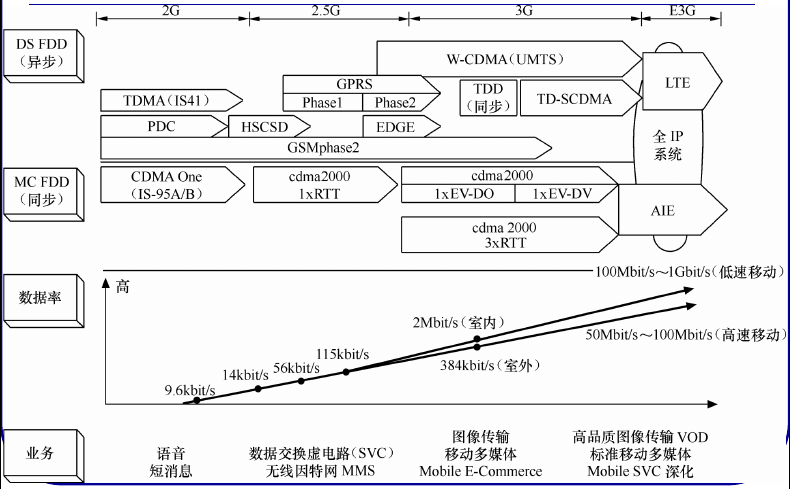
\includegraphics[scale=0.7]{移动通信系统2G_4G发展.png}
		\caption{移动通信系统发展}
	\end{figure}
	\begin{figure}[H]
		\centering
		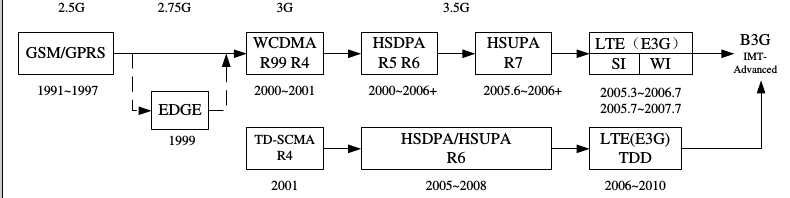
\includegraphics[scale=0.7]{WCDMA_TD-SCDMA发展.png}
		\caption{WCDMA\&TD-SCDMA发展}
	\end{figure}
	\begin{figure}[H]
		\centering
		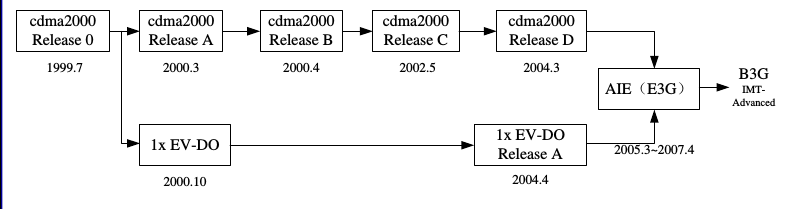
\includegraphics[scale=0.7]{CDMA2000发展.png}
		\caption{CDMA2000发展}
	\end{figure}
	
	\section{移动通信基本技术}
		\begin{figure}[H]
			\centering
			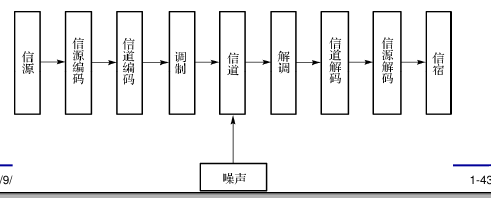
\includegraphics[scale=1]{信号传输过程.png}
			\caption{信号传输过程}
		\end{figure}
	\begin{description}
		\item[信源编码技术
		] 以提高通信有效性为目的而对信源符号进
		行的变换。
		\begin{enumerate}
			\item 波形编码
			\item 参数编码
			\item 混合编码
		\end{enumerate}
		\item[信道编码技术
		] 为了减少差错,信道编码器对传输的信息码
		元按一定的规则加入保护成分(监督元),
		组成所谓“抗干扰编码”;
		提高通信系统抗干扰能力,实现可靠通信。\\分组码、卷积码。
		\item[调制技术
		] 使要传输的信息适合于信道特征,
		达到有效、可靠的传输 。\\连续相位调制,线性调制,PSK,QPSK,DQPSK,QAM等。
		\item[电波传播特性的研究
		]  总结和建立有普遍性的数学模型,利用这些
		模型,可以估算一些传播环境中的传播损耗
		和其它有关的传播参数。
	\end{description}
	\section{蜂窝移动通信的组网技术}
	\subsection{多址接入}
	\subsubsection{什么是多址接入?}
	\textbf{定义:}移动通信系统中,使所有的用户共享
	有限的无线资源,实现不同用户不同地点同时
	通信,并尽可能减少干扰。
	\subsubsection{多路复用和多址接入区别}
	\textbf{相同点:}两者的理论基础都是\textbf{信号的正交分割原理。}\\
	\textbf{不同点:}
	\begin{itemize}
		\item \textbf{”点对点“},多路复用
		\item \textbf{"点多多点"},多址接入
	\end{itemize}
	
	\subsubsection{多址接入分类}
	\begin{enumerate}
		\item 频分多址: 第一代移动通信系统;TACS、AMPS。\\特点:
		\begin{itemize}
			\item 一个频道传送一路电话,一旦给用户分配频道,移动台和基站同时连续不断发射
			\item 信道带宽较窄。
			\item 传输速率地,码元持续时间长,与平均延迟扩展相比很大,\textbf{码间干扰不需要均衡}
			\item 系统简单,但需要一个双工器,同事需要一个RF(射频)滤波器。
		\end{itemize}
		展造成的符号间干扰低。
		\item 时分多址: 第二代移动通信系统:GSM。\\特点:
		\begin{itemize}
			\item 多个用户共享一个载波频率,分享不同时隙。
			\item 分组可以实现不连续发送。
			\item {\color{red}{由于速率较高,往往需要均衡器。}}
			\item 需要额外开销,如保护时隙,\textbf{同步}时隙等。
			\item 按照不同用户提供不同的带宽。
		\end{itemize}
		\item 码分多址: 第三代移动通信系统:IS-95 CDMA、WCDMA。\\特点:
		\begin{itemize}
			\item 通过不同的码序列来划分物理信道,信道在时间
			和频率上重合
			\item 码不但可以区分信道(walsh和OVSF),还可以区分基站(gold)或用户(m序列)
			\item  CDMA系统的许多用户共享同一频率
			\item 由于信号被扩展在一较宽频谱上,所以可\textbf{减小多
			径衰落;}
			\item 在CDMA系统中,信道数据速率很高,采用分集
			接收最大比合并技术,可获得最佳的抗多径衰落
			效果;
			\item 软切换和有效的宏分集
			\item  低信号功率谱密度
		\end{itemize}
		存在两个重要问题:
		\begin{enumerate}
			\item  多址干扰
			\item  远近效应.
		\end{enumerate}
		\item 空分多址。特点:
		\begin{itemize}
			\item 实现空间分割的基本技术就是\textbf{自适应阵列天线},在不同的用户方向上形成不同的波束。
			\item 有效地克服\textbf{多径干扰和同频道干扰}
		\end{itemize}
		\item OFDMA.正交频分多址接入
		\item NOMA,非正交频分多址接入
	\end{enumerate}
	\subsection{工作方式}
	\begin{enumerate}
		\item 单工::通信双方电台交替地进行收信和
		发信。\textbf{对讲机}。
		\item 半双工:是指通信双方中,一方使用双
		频双工方式,即收发信机同时工作;另一
		方使用双频单工方式,即收发信机交替工
		作。\textbf{基站-手机}。基站处于全双工,手机处于半双工。
		\item 全双工:是指通信双方收发信机均同时工作。收信和发信必须\textbf{采用不同的工作频率},\textbf{打电话}	\\
		双工模式:
		\begin{enumerate}
		\item 频分双工FDD:通信双方收发信可同时进行,但收信和发信分别占用两个不同的频率。
		\item 时分双工TDD:使用相同频率,但不同的时隙进行区分。
		\end{enumerate}
		两种模式的区别:
		
		\begin{itemize}
			\item TDD可灵活配置频率,\textbf{使用FDD系统不易使用的零散
			频段};但为避免与其他无线系统之间的干扰,TDD
			需预留较大的保护带,影响\textbf{整体频谱利用效率}。
			\item TDD可以通过调整上下行时隙转换点,改变上下行
			时隙比例,可\textbf{很好地支持非对称业务}。
			TDD系统\textbf{收发信道同}频,无法进行干扰隔离,速度
			越快,衰落变换频率越高,衰落深度越深;相当于
			混合行驶,容易撞车,因此必须要求\textbf{移动速度不能
			太高}。
			\item TDD接收上/下行数据时,不需收发隔离器,只需一
			个开关即可,降低设备的复
			\item 由于TDD方式的时间资源\textbf{分别分给了上行和下行,
			因此TDD方式的发射时间大约只有FDD的一半},如果
			TDD要发送和FDD同样多的数据,就要\textbf{增大TDD的发
			送功率}
			\item TDD系统上行受限,因此TDD基站的\textbf{覆盖范围明显小}
			于FDD基站。
			\item FDD模式的特点是在分离(上下行频率间隔45MHz
			190MHz等)的两个对称频率信道上,系统进行接收
			和传送,用保护频段来分离接收和传送信道。相当
			于分道行驶,比较顺畅,所以\textbf{FDD速度会更快}。
		\end{itemize}
	
		\begin{center}
			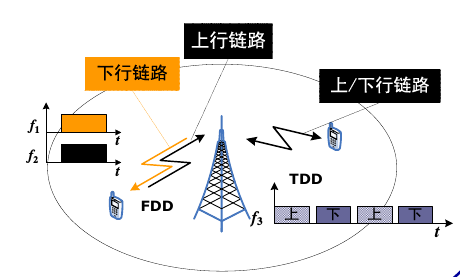
\includegraphics[scale=1]{双工模式.png}
		\end{center}
	\end{enumerate}
	\subsection{频率复用和蜂窝小区}
	\subsubsection{移动通信网的区域覆盖方式}
	\begin{enumerate}
		\item 小容量的大区制(发射功率大),基站发射功率要大,利用分集接收等技术来保证上行链路的通信质量。
		\item  大容量的小区制,(频率复用),同频干扰问题
	\end{enumerate}
	\subsubsection{区群}
	\begin{minipage}{0.4\linewidth}
	\textit{要想正多边形无空隙、无重叠地覆盖一个平面的区域,只有\textbf{正三角形、正方形和正六边形三种形状}}
	\end{minipage}
	\begin{minipage}{0.4\linewidth}
		\centering
		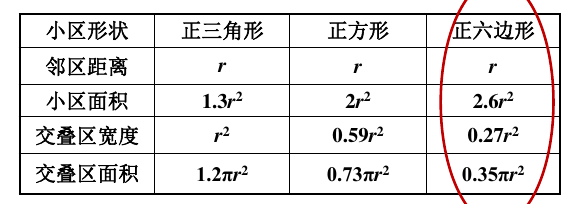
\includegraphics[scale=0.6]{三种形状方案.png}
	\end{minipage}\\
	 \textbf{定义:}共同使用全部可用频率的N个小区组成一个区群。\\
	 \textbf{特点:}
	 \begin{enumerate}
	 	\item 同一个小区,使用不同的频率。
	 	\item 不同小区,可以使用相对应的频率。
	 \end{enumerate}
 	\textbf{组成区群的小区数对应的公式}:
 	\begin{eqnarray}
 		N = i^2+ij+j^2
 	\end{eqnarray}
	一个共有S个信道的蜂窝系统(一个区群),每簇含有N个小区(一个区群),每个小区含有K个信道。则:
	\begin{eqnarray}
		S = KN
	\end{eqnarray}
	将这个簇重复M次,则信道总数为C:
	\begin{eqnarray}
	C = MS = MKN
	\end{eqnarray}
	\subsubsection{同频道距离}
	\textbf{STEPS:}
	\begin{enumerate}
		\item 首先垂直六边形的任一边延长$Max\{i,j\}$个小区。
		\item 逆时针旋转60°,在延长$Min\{i,j\}$个小区。
	\end{enumerate}

	\begin{figure}[H]
		\centering
		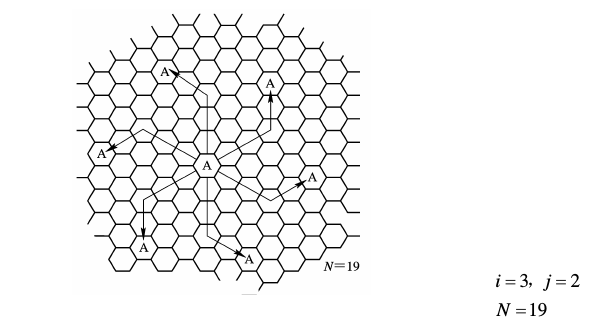
\includegraphics[scale=0.8]{通频道距离确定.png}
		\caption{通频道距离确定}
	\end{figure}
	\begin{minipage}[c]{0.8\linewidth}
			\begin{gather*}
		D^2 = I^2 + J^2 - 2IJ\cos120°	\\
		H = \frac{\sqrt{3}}{2}R	\\
		I = \sqrt{3}iR,J = \sqrt{3}jR	\\
		\Rightarrow 
		D = \sqrt{3N}R,\text{其中}N = i^2+ij+j^2
		\end{gather*} 
	\end{minipage}
	\begin{minipage}[r]{0.2\linewidth}
		\stepcounter{equation}
		(\theequation)
	\end{minipage}
	
	\subsubsection{同频干扰}
	移动台的接收载波干扰比为: \\

	\begin{gather}
		\frac{C}{I} = \frac{C}{\sum_{i=1}^{L}I_i} \notag  \\
		\frac{C}{I} = \frac{(D/R)^n}{L}=\frac{\sqrt{3N}^n}{L} 
		\label{eq:载干比}
	\end{gather}

	其中,L为同频干扰小区数,由于一般是第一层起主要作用,所以L=6(因为采用的是正六边形),则公式可改写为:
	\begin{eqnarray}
	\frac{C}{I} = \frac{(D/R)^n}{L}=\frac{\sqrt{3N}^n}{6} 
	\end{eqnarray}
	n常取4,用Q表示同频复用比例$Q = \frac{D}{R}$。注意:\textbf{\(\frac{C}{I}\)带入计算时要去分贝化}。
	\subsubsection{蜂窝系统容量}
	通常衡量
	系统容量的指标是\textbf{每小区的可用信道数来度量}:
	\begin{equation}
		n = \frac{B_t}{B_cN}
	\end{equation}
	\begin{itemize}
		\item $B_t$ 系统总带宽
		\item $B_c$ 单个小区占用的信道带宽
		\item $N$ 频率复用因子,利用\ref{eq:载干比}载干比来计算
		\begin{equation*}
			N = \sqrt{\frac{2}{3}\times \frac{C}{I}}
		\end{equation*}
	\end{itemize}
		
	\begin{description}
		\item[FDMA系统] 		

		
		\begin{equation}
		n = \frac{B_t}{B_c\sqrt{\frac{2}{3}\times \frac{C}{I}}}
		\end{equation}
		\item [TDMA系统]
		\begin{gather}
			n = \frac{B_t}{B_c^{'}\sqrt{\frac{2}{3}\times \frac{C}{I}}} \notag \\
			B_c^{'} = \frac{B_c}{m}
		\end{gather}
		\begin{itemize}
			\item 	$B_c^{'}$是等效带宽。相当于原来一个频道带宽又分给了多个时隙。
			\item  		m是每一频道包含的时隙数。
		\end{itemize}
		TDMA采用了数字技术,要求的载干比比FDMA的小,N值也比较小。
		\item[CDMA系统] 
		\begin{equation}
		n = [1+\frac{W/R_b}{E_b/I_0}\times \frac{1}{d}]\times G\cdot F
		\end{equation}
		\begin{itemize}
			\item  $E_b/I_0$
			是归一化信噪比,计算时需要\textbf{去分贝化}
			\item $W/R_b$是系统的扩频因子,即系统的处理增益。
			\item d是占空比
			\item G为扇区分区系数
			\item F信道复用系数
		\end{itemize}
	\end{description}
	\subsubsection{几种蜂窝系统的比较}
	\begin{itemize}
		\item FMDA和TDMA是频率受限系统,影响因素:频率与载干比
		\item CMDA是干扰受限系统,影响因素:扩频处理增益,信噪比,占空比,扇区分区系数,信道复用系数等。
	\end{itemize}
	\subsubsection{提高蜂窝系统容量的方法
	}
	\begin{enumerate}
		\item 	基站发射机位置
		\begin{enumerate}
			\item  中心激励小区:安置在小区的中心
			\item  顶点激励小区:安置在六边形3个间隔的顶点上 \\
			\begin{center}
			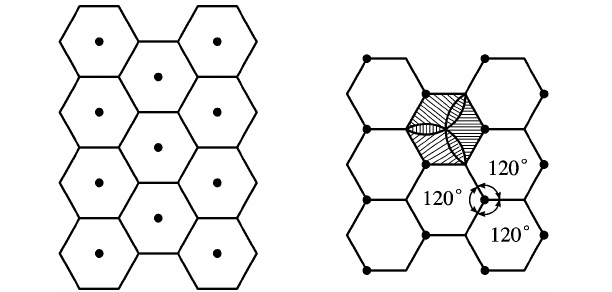
\includegraphics[scale=0.7]{基站发射机位置.png}
			\end{center}
		\end{enumerate}
		\item 小区分裂,\textbf{增加信道的复用次数}。
		\item 划分扇区,\textbf{使用定向天线减少同频干扰}。
		\item 新微小区,在微小区见运动时\textbf{不需要进行越区切换},保证覆盖范围的同时也\textbf{减小了同频干扰}。
	\end{enumerate}
	\subsection{多信道共用技术}
	\begin{itemize}
		\item 信道 --> (1)控制信道CCH,(2)业务信道THH
		\item 信道共用,原因:移动通信的频率资源十分紧缺,一个基站不可能为
		其所覆盖小区的每一个移动台预留一个专用的信道,
		而是采用信道共用的方式。
		\begin{center}
			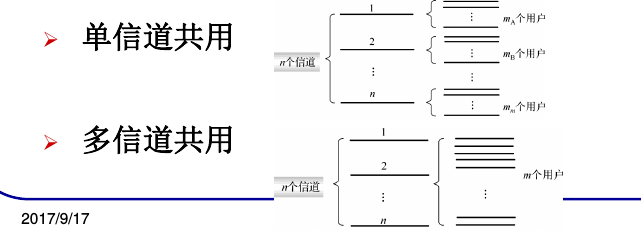
\includegraphics[width=\linewidth,height=4cm]{信道共用.png}
		\end{center}
	\end{itemize}
	\subsubsection{话务量}
	\begin{itemize}
		\item 话音业务量,用话务量描述。
		\begin{itemize}
			\item 流入话务量$A = Ct$,C为单位时间内平均发生的呼叫次数,t为每次呼叫平均占用信道时间。
			\item 完成话务量$A_0=C_0t_0$,$A_0$完成话务量,$C_0$为呼叫成功次数,t伪呼叫平均占用信道时间。
		\end{itemize}
		\item 非话音业务量,用信息流量来描述。
	\end{itemize}
	话务量是通过链路到达交换机的\textbf{总业务量}。现在要求系统能够容纳的系统用户数量,首先求解单个用户所需话务量:
	单个用户忙时话务量:
	\begin{eqnarray}
		\alpha = CTk\frac{1}{3600}
	\end{eqnarray}
	其中,C,T同上,k为集中系数,即忙时话务量对全天话务量之比。
	所以:
	n个共用信道所能容纳的总用户数:
	\begin{eqnarray}
		N = mn = \frac{A}{\alpha}
	\end{eqnarray}
	每个共用信道所能容量的用户数m:
	\begin{eqnarray}
		m = \frac{A/n}{\alpha}
	\end{eqnarray}
	n为共用信道数个数。
	\subsubsection{呼损率和爱尔兰公式}
	流入话务量-完成话务量=损失话务量。\textbf{呼损率B=}损失话务量/流入话务量:
	\begin{eqnarray}
		B = \frac{A-A_0}{A}
	\end{eqnarray}
	损失话务量越低服务质量越高,公网长取0.05,要提高B只有降低A。\\
	话务理论的经典公式-爱尔兰呼损公式:
	\begin{equation}
		B = \frac{A^n/n}{\sum_{i=0}^{n}A^i/i!}
	\end{equation}
	其中,
	\begin{itemize}
		\item B,呼损率
		\item A,流入话务量
		\item n,共用信道数
	\end{itemize}
	 信道利用率公式
	\begin{equation}
	\eta = \frac{A(1-B)}{n}
	\end{equation}


	 \textbf{用途:}\\
	 \begin{itemize}
	 	\item 计算共用信道n。
	 	\item 计算总用户量M。
	 \end{itemize}
	\subsection{网络结构}
	\begin{figure}[H]
		\centering
		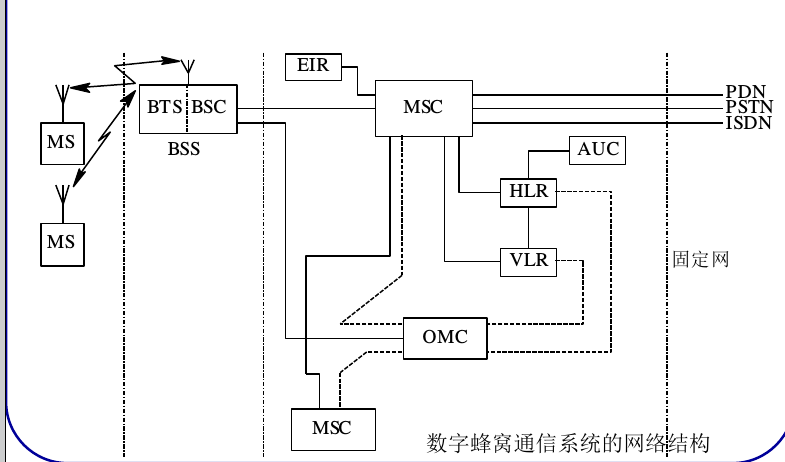
\includegraphics[width=0.8\linewidth]{网络结构.png}
		\caption{网络结构}
	\end{figure}
	\begin{enumerate}
		\item MS--移动台。如:手机,车载终端。
		\item BTS--基站收发信机。处理网络侧的无线信号收发。和MS直接交互。
		\item BSC--基站控制器。一个BSC连接1--255个BTS。
		\item MSC--移动交换中心。MSC与VLR一一对应,工程上又称为MSC/VLR。MSC的主要功能有:
		\begin{enumerate}
			\item 路由管理
			\item 业务量管理:短信,电话,流量。
			\item 计费和费率管理,为用户通信时间生成详细话单记录。
			\item 向HLR发送有关业务量和计费信息。
		\end{enumerate}
		\item VLR--访问位置寄存器,功能:
		\begin{enumerate}
			\item MS漫游号码管理。
			\item TMSI分配与管理。(临时用户移动用户表示,移动台地址)
			\item 用户参数管理
			\item 用户鉴权。
			\item HLR更新。
			\item 管理MSC区、位置(LA)区及基站区。
			\item 无线资源管理。
		\end{enumerate}
		\item HLR--归属位置寄存器。(一个用户只和一个HLR关联,即用户的SIM卡和HLR关联)
		\begin{enumerate}
			\item 管理和维护在HLR中等级注册的所有用户的参数。用户的MSISDN号码(被叫号码,如公司里的短号);;用户定制的业务信息;智能业务(VPN
			组网等);IMSI号码(SIM卡号,唯一)。
			\item 计费管理
			\item VLR更新。
		\end{enumerate}
		\item AuC--鉴权认证中心。管理用户的IMSI、密钥、加解密参数、鉴权参数。
	\end{enumerate}
	\subsection{网络的控制与管理}
	\textbf{移动性管理功能:}移动从一个位置区漫游到另一个位置
	区时,网络中的有关位置寄存器要随之对移动台
	的位置信息进行登记、修改或删除 \\
	\textbf{越区:}移动台在\textbf{通过过程中},MS从一个BTS服务区进入另一个BTS服务区,MS与原BTS之间无线链路转到MS与新BTS之间的无线链路上来。
	\subsubsection{越区切换类型}
	\begin{enumerate}
		\item 硬切换:断开与原BTS的链接,再建立和新BTS的链接。GSM
		\item 软切换:先建立与新BTS的链接,再断开和原BTS的连接。CDMA
		\item 接力切换。TD-SCDMA。
	\end{enumerate}
	\subsubsection{越区切换的判定准则}
	\begin{enumerate}
		\item 相对信号强度准则。
		\item 门限规定的相对信号强度准则。
		\item 具有滞后余量的相对信号强度准则。
		\item 具有门限规定和滞后余量的相对信号强度准则。商业
	\end{enumerate}
	\begin{figure}[H]
		\centering
		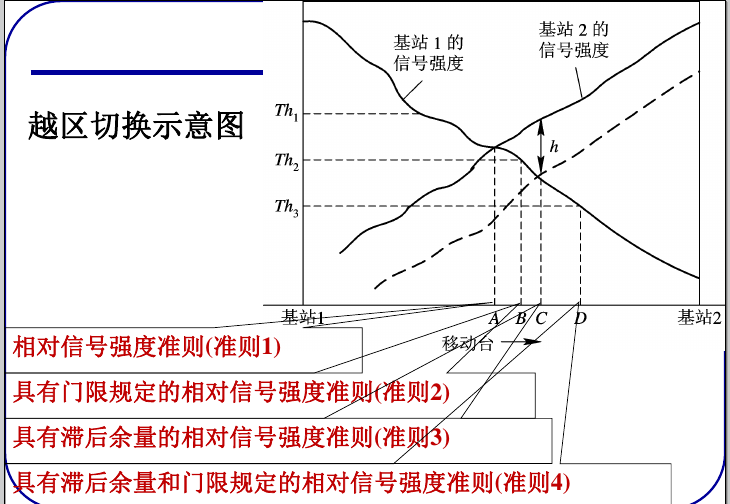
\includegraphics[width=\linewidth]{越区切换判定准则.png}
		\caption{越区切换判定准则}
	\end{figure}
	\subsubsection{越区切换的控制策略
	}
	\begin{enumerate}
		\item 移动控制,测量和判定过程全部由MS完成;
		PHS
		\item 网络控制,测量和判定过程全部由网络完成;
		AMPS
		\item 移动台辅助控制,测量由移动台来完成,判决
		由网络来完成。
	\end{enumerate}
	\subsubsection{越区切换时的信道分配
	}
	为了使得越区失败的概率尽量小,常用
	的做法是在每个小区预留部分信道专门用
	于越区切换。
	\subsubsection{位置管理}
	\begin{enumerate}
		\item \textbf{位置登记:}当用户开关机或者在位置区
		(LAI或REG\_ZONE(CDMA))之间移动或者经
		历了一个固定的时间间隔的时候,移动台需
		要向网络报告它的位置.开机登记、关机登记、基于时间登记、\\
		基于位置区变更登记.
		当一个移动终端(MT)进入一个新的RA时, 位置
		登记过程分为三个步骤:
		\begin{itemize}
			\item  在管理新RA的新VLR中登记MT;
			\item  修改HLR中记录服务该MT的新VLR的ID;
			\item 在旧VLR和MSC中注销该MT。
		\end{itemize}
		\textbf{具体过程:}\\
		\begin{figure}[H]
			\centering
			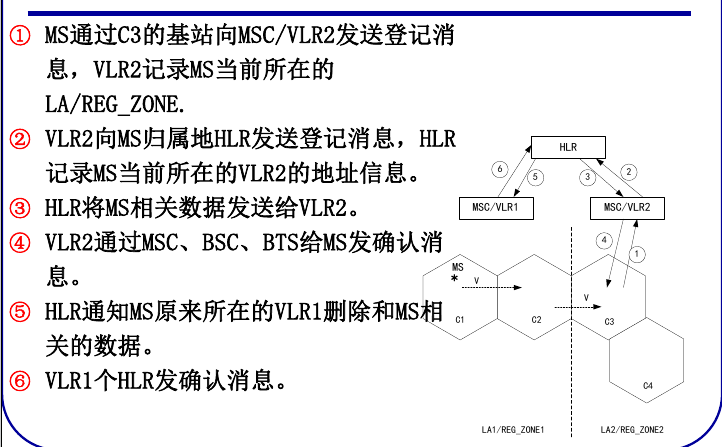
\includegraphics[width=\linewidth]{位置区切换过程.png}
			\caption{位置区切换过程}
		\end{figure}
	\item 呼叫传递:
	\begin{figure}[H]
		\centering
		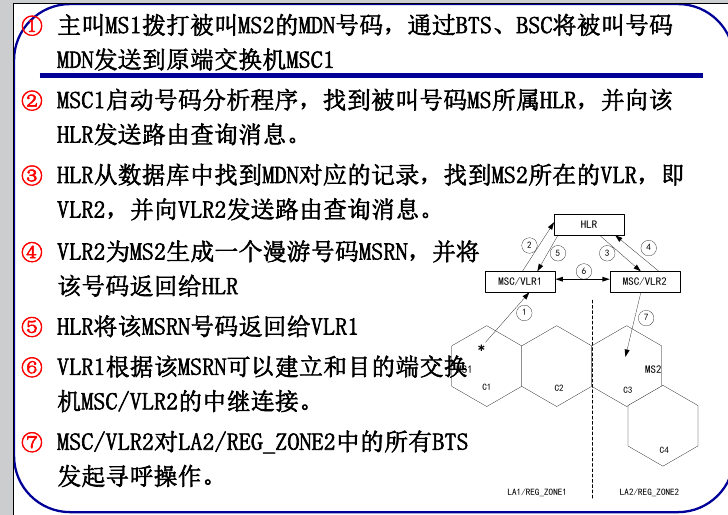
\includegraphics[width=\linewidth]{呼叫传递.png}
		\caption{呼叫传递过程}
	\end{figure}
	\end{enumerate}

%	
\section{报告}
\subsection{通信网的组成要素}
\question{当今典型网络的终端设备、设备线路、交换设备,主要设备的工作原理和功能}
\begin{description}
 	\item[终端设备] 主要功能是把待传送的信息和在信道上传送的信号之间的相互转换。
	\begin{itemize}
		\item 发送传感起来感受信息和接受传感器将信号恢复称能被利用的信息
		\item 能处理信号的设备使之能与信道匹配
		\item 能产生和辨别网内所需的信令或协议,以便相互联系和应答
	\end{itemize}
	\item[设备线路] 传输线路,踏实电磁波传输的路径。通常分为无界传播和导引传播。
	\begin{enumerate}
		\item\textbf{无线信道} 传输通道主要自由空间,需要发射机、发射天线、接受天线和接收机。
		\begin{enumerate}
			\item \textbf{长波线路}300$kHz$以下。沿地面尤其是海岸的传播损耗小。一般用于航海系统中
			\item \textbf{短波线路}3$MHz$-30$MHz$。传播损耗已较大,但利用地球上空电离层反射,可进行远距离通信。
			\item \textbf{微波线路}\ 作为通信网的信道的主要方式是中继线路或接力线路。
		\end{enumerate}
		\item \textbf{有线信道} 电磁波是沿道题传播的,而且通常是能构成直流通路,适宜与基带传输。包括\textbf{架空明线、平衡电缆、同轴电缆、波导传输。},除了有线线路还需要增加\textbf{增音器和均衡器}。
	\end{enumerate}
	\item[交换设备] 终端设备和信道是构成通信系统的必要设施,除此之外,还需要交换设备
	\begin{enumerate}
		\item \textbf{电路交换}
		\item \textbf{分组交换}\ 分组交换在网路资源利用上比电路交换方式好,但总要引入一定延时,所以对实时要求高的如电话通信不利。
		\item \textbf{多址接入}\ 上两者都需要讲交换信息传送到一个交换点或转接站。引入多址接入可使哥哥用户直接接送到线路上去。
	\end{enumerate}
\end{description}
\question{电话网与计算机通信网的不同}
\begin{enumerate}
 	\item 传统电话网使用电路交换方式,而计算机通信网多使用分组交换方式或虚电路方式。
 	\item 电话网对交换的实时性要求高,但对准确率要求相对较低。计算机通信网则对实时性要求相对低,准确率要求高。
 	\item 电话网传输速率相对计算机通信网普遍较低。
\end{enumerate}
\question{通信网的约定的概念,电话网的约定、因特网的约定}
	\begin{enumerate}
		\item \textbf{通信网的约定}\ 网内使用的一种``语言'',用他们来协调网的运行,达到互通、互控和互换的目的。
		\item \textbf{电话网的约定}\ 电话信令
		\item \textbf{因特网的约定}\ 计算机通信协议
	\end{enumerate}
\question{通信网的质量标准及传输标准}
 	\begin{enumerate}
 		\item \textbf{质量标准}\ 质量决定于信道的比特误码率
		\begin{enumerate}
			\item 接续质量,受网资源的容量和可靠性限制,主要靠增加网资源来提高
			\item 信息质量,受终端额信道的失真和噪声等限制,因信息类型的不同而不同。
		\end{enumerate}
		\item \textbf{传输标准}\ 规定了信道接口的一系列参数。
 	\end{enumerate}


%%	\chapter{移动信道的传播特性于模型}
\section{无线电波传播方式
}
移动通信使用\textbf{甚高频(VHF)}和\textbf{特高频(UHF)}等频段传输。
\begin{description}
	\item[VHF:] 1--10m,30--300MHZ
	\item[UHF:] 10--100CM,300MHZ--3GHZ
\end{description}
当频率f > 30 MHZ时,传播通路主要有:直射波、反射波、地表面波。
\subsection{直射波}
直射波传播,可按自由空间传播来考虑。
\begin{description}
	\item[条件:] 自由空间传播是指天线周围为无
	限大真空时的电波传播
	\item[现象] 不发生反射、折射、绕射、散射
	和吸收等现象,但电波经过一段路径传播之
	后,能量仍会衰减,这是由电磁波能量扩散而引起的传播损耗
	(弥散损耗或称为自由空间传播损耗)。
	\begin{eqnarray}
	L_{fs}(dB) = 32。44 + 20lg_d(km)+20lg_f(MHZ)
	\end{eqnarray}
\end{description}
传播接受能量排序:直射>(反射、绕射)>散射。
\subsection{反射波}
物体尺寸比传输波长大得多(如地面,墙面),则容易发生镜面反射。
\subsection{绕射波}
尖利边缘(山丘)。

余隙:障碍物顶点P到直射线TR的距离,称为菲涅尔余隙。阻挡时为负(即当障碍物高于TR线时),反之为正。\textbf{附加损耗可通过查表得到},该损耗和相对余隙$x/x1$有关,其中\(x1\)第一菲涅尔半径,x为余隙长度。
\begin{eqnarray}
x_1 = \sqrt{\frac{\lambda d_1d_2}{d_1+d_2}}
\end{eqnarray}
\subsection{散射}
比传输波长小的多的物体(粗
糙表面、不规则物体),并且单位体积内阻挡体的个数很堵的情况。
\subsection{反射、绕射和散射的关系}
\begin{tabular}{|c|c|}
	\hline
		&阻挡体	\\
		\hline
		反射	&	比传输波长大的多的物体(地
		面、墙面)	\\
				\hline
		绕射	&	尖利边缘(山丘)\\
				\hline
		散射	&	比传输波长小的多的物体(粗
		糙表面、不规则物体)	\\
				\hline
\end{tabular}

\section{移动信道的特性
}
\subsection{传播路径与信号衰落
}
无线电波的传播表现出几种主要传播方式为:
直射、反射、绕射和散射,以及它们的合成。\\
无线电波通过时变信道,主要表现出4种效
应为:\textbf{多径效应(由于地理环境的影响,接受的信号是各路径的矢量和、多普勒效应(运动造成频谱扩撒)、阴影效应(由于障碍物的阻挡,在电磁传播的接受区域内产生传播半盲区)和远
近效应(近处无用强信号抑止远处有用弱信号。}
\subsubsection{两种衰落及其比较}
\begin{itemize}
	\item 大尺度衰落
	\item 小尺度衰落
\end{itemize}
\begin{tabular}{|c|m{6cm}|m{6cm}|}
	\hline
		&大尺度衰落	&小尺度衰落		\\
	\hline
	描述
	& 长距离上信号强度的缓慢变化,采用平均路径损耗和相对均值的对数正态分布变化来描述	&	短距离上信号强度的快速变化,采用信号的时延拓展和信道的时间变化	\\
	\hline
	原因	&	信道路径上的固定障碍物阴影	&	多径传播和收发两端的相对运动\\
	\hline
	影响	& 业务覆盖区域	&	信号的传输质量	\\
	\hline
\end{tabular}
\subsection{多径效应与瑞利衰落
}
移动无线信道的主要特征是\textbf{多径传播}。接
收点所获信号是多个路径来的信号的叠加。\\

假设:收发间的多条路径各参数(幅度,方向角)统计独立,且收发间{\color{red}{\textbf{不存在直射波}}},这多径接受信号的{\redbf{幅度}}服从{\redbf{瑞丽分布}},{\redbf{如果存在直射波}},则服从{\redbf{莱斯分布}}。\\
重要结论:一个均值为0、方差为 的平稳高
斯窄带过程,它的\textbf{包络}的一维概率密度服从\textbf{瑞
利分布},\textbf{相位}的一维概率密度分布是\textbf{均匀分布}。
\subsection{三类主要的快衰落
}
\begin{description}
	\item[多径效应] 在时域上引起信号的时延扩展,使得接
	收的信号分量展宽,相应地在频域上规定了相关带宽
	性能。当信号带宽大于相关带宽时就会发生频率选择
	性衰落。
	\item[多普勒效应] 在频域上引起频谱扩展,使得接收的
	信号产生多普勒频展,相应地在时域上规定了相关时
	间。多普勒效应产生的衰落是时间性选择衰落。
\end{description}
\begin{enumerate}
	\item 时间选择性衰落,在不同的时间,信道衰落特性
	不一样,这种衰落会造成信号的失真。由于移动台的高速运动在频域引起\textbf{多普勒频移},相应地其时域波形产生时间选择性衰落。(可由频率变化了$\Delta f$,利用逆傅里叶变换得到时域式子,在取幅度模即可知道限制了时间宽度,所以称为时间选择性衰落,相关时间$\Delta t = \frac{1}{\Delta f}$,$\Delta f${\color{red}{基带信号带宽})}。\textbf{为保证不在时间轴上失真,必须保证传输符号速率远大于相关时间\footnote{在一段时间间隔内,到达信号具有很强的相关性,即信道特性在此时间段内没有发生明显的变化}的倒数,即$R_s$越大越好,发送时间的间隔$\Delta t$越小越好}。
	\item 频率选择性衰落,指在不同频段上衰落特性不一样,由于\textbf{多径传播}造成在时域的时延扩散(引起ISI),引起各网
	络对不同频率的信号衰减也不同,这使得接收点合成
	信号的频谱中某些频率分量衰减特别厉害,产生频率
	选择性衰落(可由时间变化了$\Delta t$,利用傅里叶变换得到频率式子,再取幅度模可知道限制了频率宽度,所以称为频率选择性衰落,$\Delta f = \frac{1}{\Delta t}$,$\Delta t$ 多径时延。工程上相关带宽\footnote{在频率间隔靠得很近的时候,到达信号具有很强的相关性,这个频率间隔就称为相关带宽}为$\Delta f = \frac{1}{2\pi \Delta t}$)。推导可见下图
	{
		\begin{figure}[h!]
			\centering
			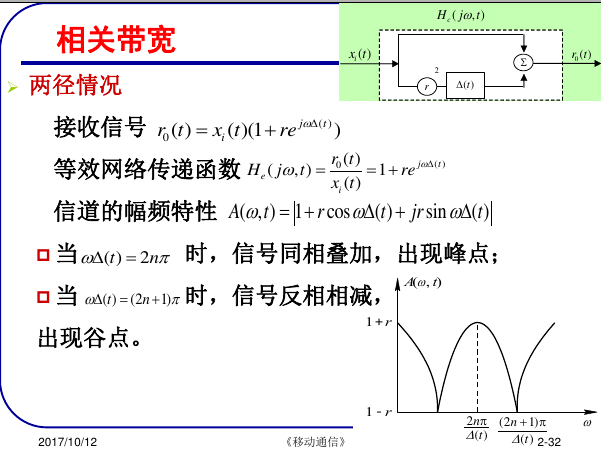
\includegraphics[width=0.7\linewidth]{figures/相关带宽退到.png}
			\caption{}
			\label{fig:}
		\end{figure}
		
}
	\item 空间选择性衰落,相关距离\footnote{在一定的空间距离,信道冲击响应能保证一定的相关度,这个空间距离就是相关距离(通长上就是接受天线防止的距离)}。
\end{enumerate}
\subsection{ 慢衰落特性和衰落储备
}
\subsubsection{满衰落}
定义:无线通信中,一般把由于距离引起的路径损耗和由于地形遮挡引起的阴影衰落统称为慢衰落,其衰落周期为秒级。
\begin{itemize}
	\item 天气引起的变化,更慢,小时或天级。
	\item 近似服从\textbf{对数正态分布}
\end{itemize}
\subsubsection{衰落储备}
 为了防止因衰落(包括快衰落和慢衰落)引
起的通信中断,在信道设计中,必须使信号的
电平留有足够的余量,以使中断率R小于规定
指标。这种电平余量称为衰落储备。\\
衰落储备大小决定于地形、地物、工作频率和要求的通信可靠指标(可通率T= 1-R)。\\
衰落储备可通过查表得到。

\section{陆地移动信道的传输损耗
}
\subsection{地形的分类
}
\begin{description}
	\item[中等起伏地形]地
	面起伏高度不超过20m。
	\item[不规则地形] 其余地形。
\end{description}
\textit{移动台天线的有效高度h 总是指天线在当地地面
	m上的高度。
}
\subsection{地物(地区)分类}
\begin{itemize}
	\item 市区
	\item 郊区
	\item 开阔地
\end{itemize}
\subsection{中等起伏地形上传播损耗的中值
}
奥村模型:适用范围:频率150MHZ ~1500MHZ,基
地站天线高度为30~200米,移动台天线高度为1~10
米,传播距离为1~20千米的场强预测。\\

基准中值:在计算各种地形、地物上的传播损耗
时,均以\textbf{中等起伏地}上的\textbf{市区},在\textbf{标准天
线高度,基站天线200m,移动台天线3m}下的损耗中值或场强中值作为基准,
称作基准中值或基本中值。其余情形将在
此基准上作修正。修正因子为实际场强中
值与基准场强中值之差。

\subsubsection{中等起伏地形损耗中值计算}
\begin{itemize}
	\item 自由空间损耗。+
	\item 传播损耗基准中值$A_m$(相对于自由空间的中值损耗),f,d越大$A_m$越大。+
	\item 基站天线高度增益因子 $ H_b $。天线越高,其值越大(天线越高,损耗越小)。-
	\item 移动台天线高度增益因子$ H_m $。天线越高,其值越大(天线越高,损耗越小)。-
	\item 街道走向修正因子 $ k_a $。纵向(与传播方向平行),大于0,横向(垂直),小于0。-
\end{itemize}
\begin{equation}\label{key}
L_t = L_{fs} + A_m - H_b - H_ -k_a
\end{equation}

\subsubsection{郊区和开阔地损耗的中值
}
\begin{equation}\label{key}
L_{\text{郊区}} = L_{\text{市区}} - K
\end{equation}
K为地形修正因子。\\
中等起伏地市区中接收信号的功率中值$ P_p $
\begin{equation}\label{key}
 P_p = P_0 - A_m + H_b + H_m
\end{equation}
$ P_0 $发送功率,其余地形技术算,即加上相应的地形修正因子。
\begin{equation}\label{key}
 P_p = P_0 - A_m + H_b + H_m+K_T
\end{equation}

\section{传播模型}
\begin{figure}[H]
	\centering
	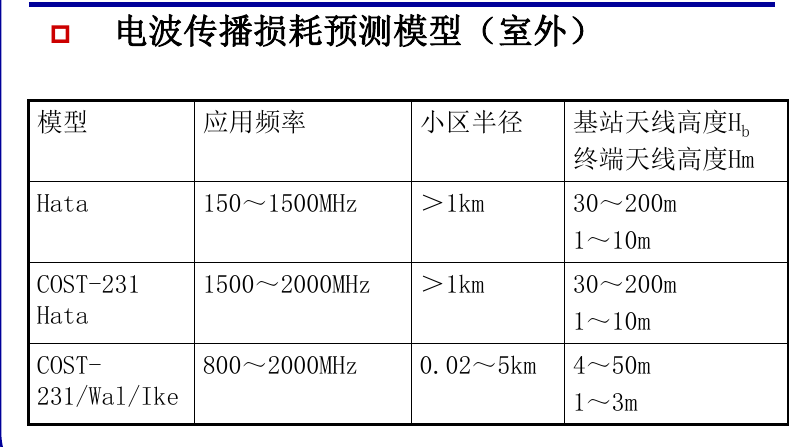
\includegraphics[width=0.7\linewidth]{figures/传播模型}
	\caption{}
	\label{fig:}
\end{figure}

%	\chapter{抗衰落技术}
\section{抗衰落}
\subsection{传输中的损耗}
\begin{itemize}
	\item 阴影效应 →通信范围
	\item 多径效应,多普勒效应。衰落 通信质量
	\item 噪声和干扰,误码。通信质量
\end{itemize}
\subsection{抗衰落措施
}
\begin{enumerate}
	\item 信道编码→减小信道噪声或干扰
	\item 扩频技术→减小多径干扰
	\item 分集→减小衰落深度和衰落持续时间
	\item OFDM(均衡技术)→减小码间干扰
	\item  MIMO(空间分集)→克服衰落,降低误码率
\end{enumerate}

\section{分集技术}
定义:接收端对它收到的多个衰落特性\textbf{互相独立(携带同一信息)}的信号进行\textbf{集中}处理,以降低信号电平起伏的办法。\\
{\centering \textbf{分散传输} \hspace{3cm} \textbf{集中处理}}
\subsection{分集技术的分类}
\begin{description}
	\item[宏分集“基站分集”] 将多个基站设置在不同的地理位置上和不同的方向上,移动台可和其中信号最好的一个基站进行通信。它能克服\textbf{由于阴影效应或地形影响而产生的慢衰落}\item[微分集] 在同一场地采用多副天线或多
	个频率或多种极化等方法接收和处理由多条路
	径传来的信号。移动台和基站都可使用这种技
	术。(空间、频率、极化、场分量、角度及时间),克服\textbf{快衰落}。
\end{description}
\subsubsection{空间分集}
原理:空间分集的依据在于快衰落的空间独立性。\\当两个位置的距离大于一定程度,则两处的信号衰落是不相关的。在频率较高时($ f \ge 800MHz$,容易实现空间分集。
\subsubsection{时间分集}
原理:同一信号在不同的时间区间多次重发,只要
各次发送的\textbf{时间间隔足够大},那么各次发送信号所出
现的衰落将是\textbf{彼此独立}的。\\
实现:其重发时间间隔 $\Delta T \ge \frac{1}{2fm} = \frac{1}{2(v/\lambda)}$,用于\textbf{克服多普勒效应引起的信号衰落现象}(所以移动台静止时,v=0,时间分集不起作用)。 
\subsubsection{频率分集}
原理:相干带宽之外的频率上不会出现同
样的衰落
实现:多个载频上传送信号,载频间隔大
于相干带宽$ B_c = \frac{1}{2\pi\Delta} $
\subsubsection{极化分集}
原理:两个不同极化的电磁波具有独立的衰
落特性。\\
实现:收发端用不同极化的天线分别发送和
接收信号,以获得分集效果。\\
极化分集是空间分集的一种特殊情况。将射频功率分给两个不同的极化天线,所以发射功率要损失3db。

\subsection{合并技术}
多路接受信号的加权求和。
\subsubsection{选择式合并SC}
在多路信号中选择信噪比最高的支路作为输出,即在多个加权系数中,只有一个伪1,其余为0.
\subsubsection{最大比值合并MRC}
最大壁纸合并将各路信号加权后合并。在信号合并前对各路载波相位进行调整使之同相,然后相加。\\
各路加权系数$ a_k $与信号包络$ r_k $成正比,于噪声$ N_k $成反比。这是\textbf{最佳的合并方式}。
\begin{equation}\label{key}
a_k = \frac{r_k}{N_k}
\end{equation}
所以合并信号为:
\begin{equation}\label{key}
r_R = \sum_{k=1}^{M}a_kr_k = \sum_{k=1}^{M}\frac{r_k^2}{N_k}
\end{equation}
\subsubsection{等增益合并EGC}
。无需对信号加权,
各支路的信号是等增益相加的。
\begin{equation}\label{key}
r_R = \sum_{k=1}^{M}r_k
\end{equation}
\subsection{合并技术性能分析于比较}
最大比值合并 > 等增益合并 > 选择式合并\\
合并增益D(M)与分集支路数目(M)
之间的关系:
\begin{figure}[H]
	\centering
	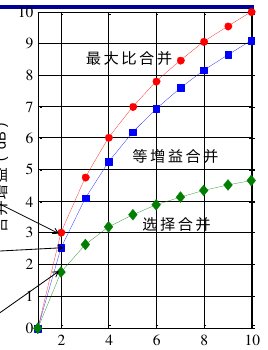
\includegraphics[width=0.7\linewidth]{figures/hebingbijiao.png}
	\caption{}
	\label{fig:}
\end{figure}
\section{信道编码技术}
\subsubsection{一些理论}
信道编码是为了保证信息传输的可靠性、提高传输质量而设计的一种编码。\\
通常分为\textbf{分组码}和\textbf{卷积码}。\\
\textbf{定义:} 在信息码元中增加一些冗余码元,用来在接收端
检测或纠正在有噪信道中引入的误码\\
码字:信息码元于冗余码元一起构成的消息块称为码字。\\
码距:对应位不同的个数,又称为汉明距。信道编码的实质就是\textbf{增加码距,码距代表了纠检错能力}\\
码距于纠检错能力的关系:
\begin{itemize}
	\item 检测e个错误:最小码距d0$\ge$e+1
	\item 纠正t个错误:最小码距d0$\ge$2t+1
	\item 纠正t个错误,发现e个码位错误:最小码距d0$\ge$t+e+1
\end{itemize}
\subsubsection{信道编码分类}
\begin{itemize}
	\item 按码组功能分:检错码和纠错码
	\item 按加入冗余码元方式:线性码和非线性码
	\item 按码组结构分:分组码和卷积码
	\item  按纠错能力分:纠随机错和纠突发错
	
\end{itemize}
性能指标:编码效率,编码增益,编码延时,编译码器的复杂度
\subsubsection{应用}
\begin{itemize}
	\item GSM,IS-95,卷积码
	\item 3G,卷积,Trobo
\end{itemize}
\subsubsection{线性分组码}
主要考虑CRC循环冗余校验,用于误码检测。表示为(n,k)码,k为输入,n为输出,编码效率R = k/n\\
生成方式:
\begin{figure}[H]
	\centering
	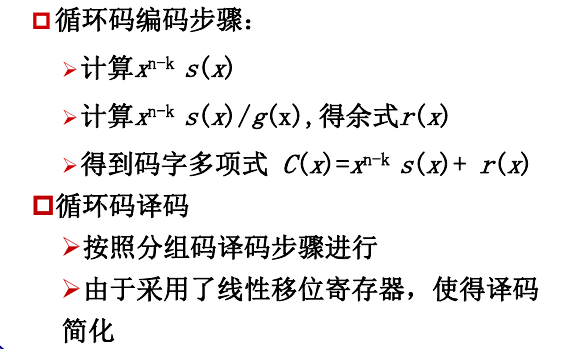
\includegraphics[width=0.7\linewidth]{CRCshengcheng.png}
	\caption{}
	\label{fig:crc}
\end{figure}
例题:
\begin{figure}[H]
	\centering
	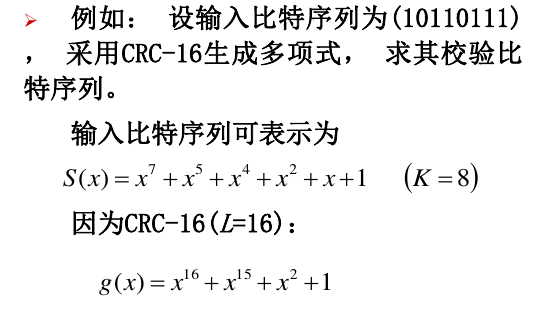
\includegraphics[width=0.7\linewidth]{CRC1.png}	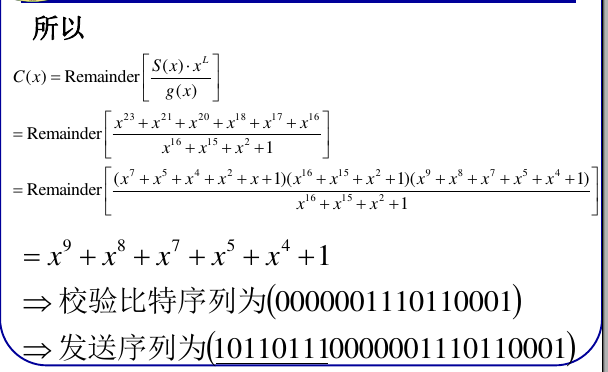
\includegraphics[width=0.7\linewidth]{CRC2.png}
	\caption{}
	\label{fig:crc1}
\end{figure}
\textbf{简便算法:}
\begin{figure}[H]
	\centering
	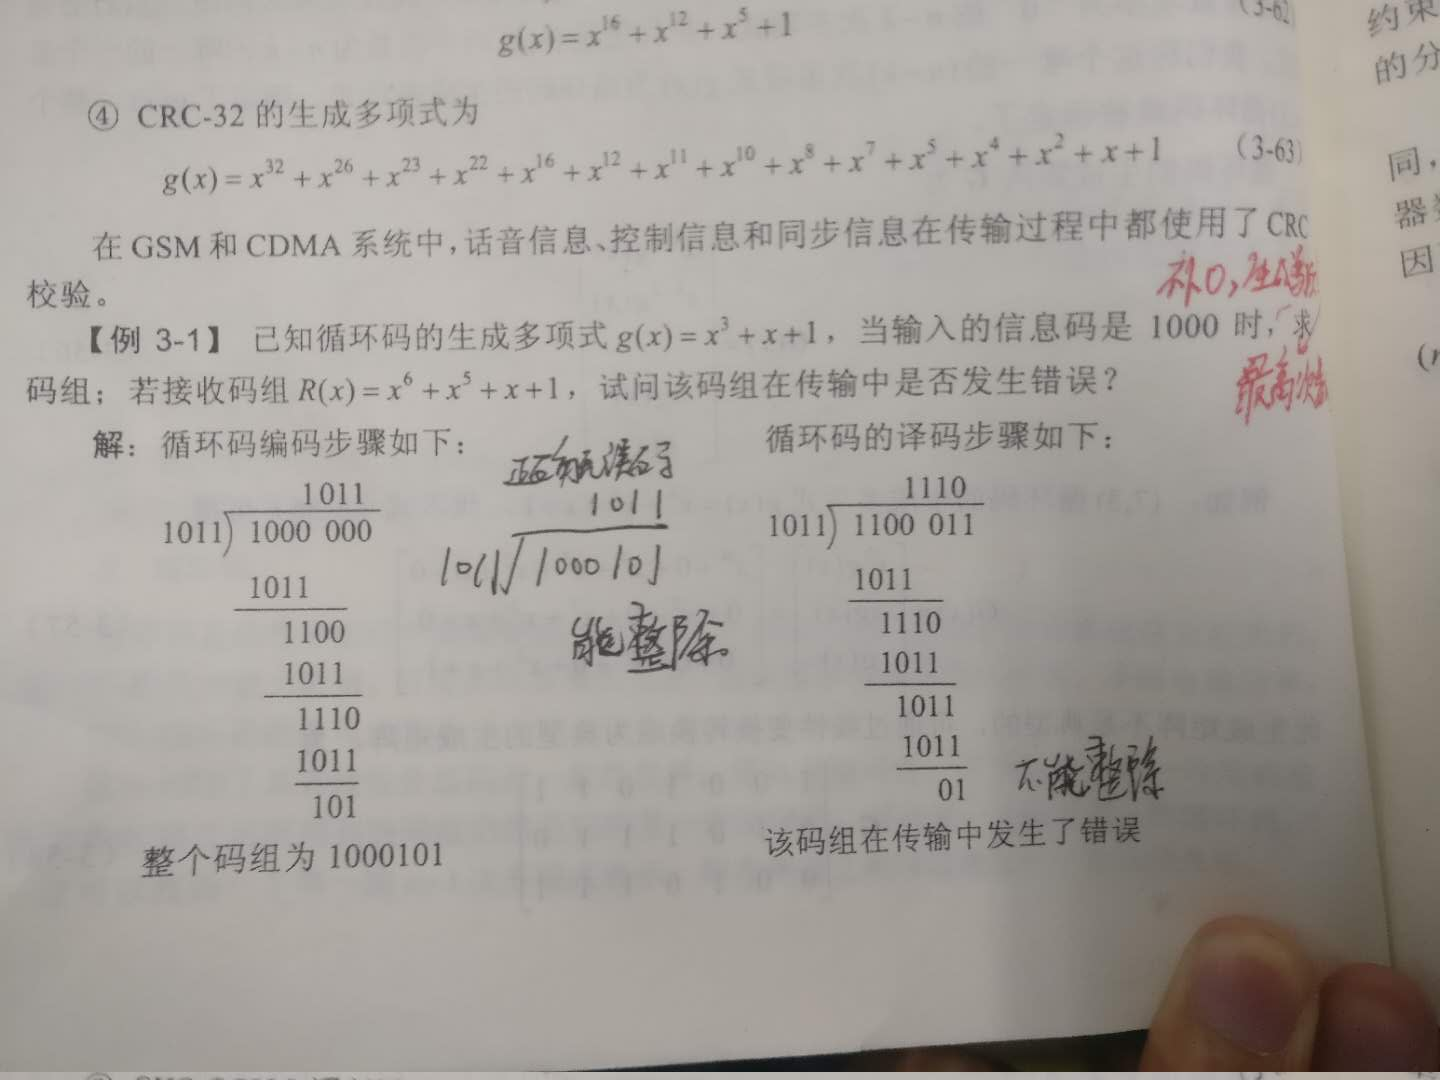
\includegraphics[width=0.7\linewidth,height=7cm]{CRC3.jpeg}
\end{figure}
验证是否出现误码,将接收到的序列除以生成多项式,整除则(可能)无误码,否则有误码。
\subsection{卷积码}
卷积码的监督码元与当前码元和前若干码
元有关。表示为(n,k,m),m为寄存器的个数。约束长度l = m+1,编码效率R=k/n。\\
为什么要称为卷积码?采用单位冲击信号输入后,得到各支路的冲激响应,将输入于各支路的冲击响应做卷积运算可得到各支路的信号输出。
\subsubsection{卷积码的描述}
\begin{enumerate}
	\item 解析法,离散卷积法、码生成多项式法、生成矩阵、
	\item 图形法,状态图、树图以及网格图
\end{enumerate}
\subsubsubsection{图解法}
\begin{description}
	\item[状态图] 圈内为寄存器状态,单斜杠前为输入,后为输出,箭头方向为寄存器转移方向。如:
	\begin{figure}[H]
		\centering
		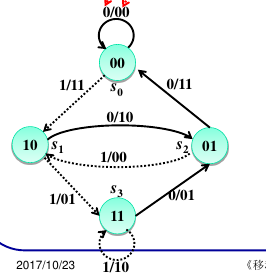
\includegraphics[width=0.7\linewidth]{zhuangtaizhuanyi.png}
		\caption{}
		\label{fig:}
	\end{figure}
	\item[网格图] 把状态图沿时间轴展开
	\begin{figure}[H]
		\centering
		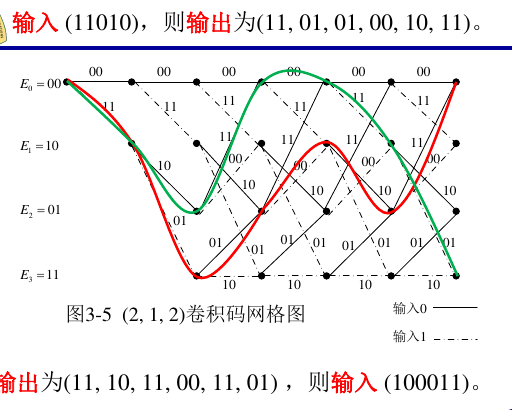
\includegraphics[width=0.7\linewidth]{wanggetu.png}
		\caption{}
		\label{fig:}
	\end{figure}
	维比特译码。
	\item [树图]
\end{description}
\subsubsection{卷积码在蜂窝移动通信系统中的应用}
所有分叉后又合并的任一长度路径中的最小距离称为自由距离df,其纠错能力为$ t = \frac{|d_f -1 |}{2} $。\\
在GSM系统中,使用上述两种编码方式,首先使用CRC编码,在对全部比特做卷积编码。\\
半速率信道编码的自由距离大于全速率信道的自有距离(GSM),反向信道编码的自由距离大于正向信道的自由距离(WCDMA),因此反向信道和半速率信道右更强的抗噪声干扰能力。
\subsection{交织编码}
交织编码的作用是改造信道,其实现方式有\textbf{块
交织,帧交织,随机交织,混合交织}等等。将一个有记忆的突发信道改造成一个随机独立的差错信道。在交织和去交织过程中会产生附加
处理时延。它本身并不具备信道编码检、纠错
功能,仅起到信号预处理的作用。\\
几个名词:
\begin{description}
	\item[交织深度
	] 交织前相邻两符号在交织后的间隔距离
	\item[交织宽度:
	] 交织后相邻两符号在交织前的间隔距离
	\item [交织延迟
	]每个符号从交织器输出时相对于输入交
	织器时的时间延迟
	
\end{description}
对于一个m$\times$n的交织阵列,如果按照\textbf{行写入,列写出},那么交织深度为m,交织宽度为n。\\
要求:交织深度大于相干时间---\textbf{时间分集,是一种时间隐分集技术}
\subsubsection{交织的作用}
交织 + 信道编码 <--> 衰落\\
\vspace{1cm}
交织常与重复或信道编码相结合,是一种对
抗突发错误的时间分集形式,信道编码技术更易于纠正随机错误,交织技
术可以在把信道中的突发错误分散成随机错误;
而衰落是移动通信中引发突发错误的主要因素。

\subsection{Turbo码}
Turbo码巧妙地将\textbf{卷积码}和\textbf{随机交织器}相结合,
采用软输入/输出译码器,可以获得接近Shannon编码
定理极限的性能。但因它存在时延,故主要用于\textbf{非实
时的数据通信}中。

\section{扩频通信}
扩频通信是利用与传输数据(信息)\textbf{无关}的扩频
函数对传输信号扩展频谱,在接收机中利用\textbf{相同}的扩
频函数对接收信号进行同步相关接收、解扩及恢复原
始信息。\\
特征:
\begin{itemize}
	\item 传输带宽远大于被传送信息的原始带宽;
	\item 传输带宽主要由扩频函数决定,扩频函数是不
	可预测的伪随机的宽带信号;
	\item 接收端中用与发射端扩频函数同步的副本实现
	相关解扩。
	
\end{itemize}
\subsection{扩频理论依据}
\textbf{香农定理}:在高斯白噪声干扰条件下,设信
号带宽为B(Hz),信道输出信号平均功率为S
(W),输出加性高斯噪声功率为N(W),则该
通信系统的信道容量C(bit/s)为:
\begin{equation}\label{key}
C = Blog_2(1+\frac{S}{N})
\end{equation}
说明:
\begin{itemize}
	\item 只要信源的信息传输速率Ri小于等于信道容量,即Ri  C,
	则总可以找到一种编码方式实现信号的无差错传输;
	\item 若传输速率大于信道容量,则不可能实现信号的无差错传
	输。
\end{itemize}
扩频信号频谱增加带宽可以换取信噪比的降
低,从而提高了通信的抗干扰能力,实现强干
扰环境下可靠安全的信息传输。\\
两个重要的结论:
\begin{itemize}
	\item 扩频信号频谱增加带宽可以换取信噪比的降
	低,从而提高了通信的抗干扰能力,实现强干
	扰环境下可靠安全的信息传输。
	\item 如果信号的总能量不变,则频谱的展宽势
	必使各谱成分的幅度下降,即功率谱密度降低。
	
\end{itemize}
\subsection{主要工作方式}
\begin{itemize}
	\item 直接序列扩频
	\item 跳变频率扩频
	\item 跳变时间扩频
	\item 宽带线性调频
	\item 混合方式
\end{itemize}
\subsection{主要性能参数}
\subsubsection{扩频处理增益}
\begin{equation}\label{key}
G_p = \frac{SNR_{out}}{SNR_{in}} =10log\frac{SNR_{out}}{SNR_{in}} (db)=  10log\frac{B_{\text{扩频后}}}{B_{\text{扩频前}}} =10log \frac{R_c(\text{伪随机序列发送速率})}{R_b(\text{基带速率})}
\end{equation}
$ G_p $表示了信噪比的改善程度
\subsubsection{干扰容限
}
在保证系统正常工作的条件下
(系统输出信噪比一定),接收机能够承受的干扰信
号比有用信号高出的分贝(dB)数,用M表示,其数学
式为:
\begin{equation}\label{key}
M = G_p - [L_s + (\frac{S}{N}_{out})]dB
\end{equation}
$ L_s $路径传输损耗。\\
干扰容限反映了扩展频谱系统接收机能在多大干
扰环境下正常工作的能力和可能抵抗极限干扰的强度。\\
例:
个扩频系统的处理增益为35dB。要求系
统在误码率小于l0-5时,信息数据解调的最小的
输出信噪比(S/N)out<10dB,系统内部损耗Ls=
3dB,则系统的干扰容限为:
\begin{equation}\label{key}
M = 35 - (3+10) = 22db
\end{equation}
所以系统能够接受,干扰输入电平比扩频信号功率电平高22dB的范围内工作,即接收端输入SNR$\ge$-22dB。
\begin{align*}\label{key}
10logN &- 10logS  \le 22	\\
10logS & \ge 10logN - 22 
\end{align*}
\text{噪声最小为0,所以扩频信号功率电平大于-22dB}
\subsection{伪随机序列
}
为伪噪声序列(PN序列):重复产生和处理,具有\textbf{随机}序列基本特性的\textbf{确定}序列。\\
用作地址码时,要求\textbf{尖锐的自相关,小的互相关}。

\subsubsection{m序列}
最长线性反馈移位寄存器序列,m序列。\\
特征多项式:
\begin{equation}\label{key}
f(x) =  \sum_{r = 0}^{m} = C_rx^r,\text{其中}C_0 = 1,C_m = 1。
\end{equation}
\begin{itemize}
	\item 序列是由多级移位寄存器或其他延迟元件通过线
	性反馈产生的最长的码序列。
	\item 在二进制移位寄存器发生器中,若n为级数,则所
	能产生的最大长度的码序列为$ N=2^n-1 $位,其中等于$ 2^n-1 $的即为m序列。
	\item m序列发生器中,并不是任何抽头组合都能产生m
	序列,需要由本原多项式生成。
\end{itemize}
\textbf{性质:}
\begin{description}
	\item[均衡特性] 在m序列中一个周期内“1”的
	数目比“0”的数目多 1位;
	\item[移位相加性] m序列和其位移序列模2加后仍为m序列
	\item[m序列相关特性] $ R_{a,b}(n) = \frac{A-D}{A+D} $A为相同位数,D为不同位数。\\其自相关函数可表示为
\[ 	 R_{a,a}(n)= \begin{cases}
		1,n=lN\\
		-1/N,其余n
	\end{cases} \]
\end{description}
\textbf{m序列的功率谱:}\\
功率谱具有抽样函数的$ Sa^2(x) $包络,其带宽取决于码元长度。

\subsubsection{Gold码}
性质:
\begin{itemize}
	\item 长度为N的一个优选对可以构成N个Gold码,
	这N个Gold码加上m1和m2,共\textbf{N+2}个码。它们之中
	任何两个码的周期性互相关函数也是三值函数(优选对的性质,即满足优选对的序列,其平移相加后的自相关函数最多有3个值)
	\item  Gold码的个数比m序列数多得多。1对m级移位寄存器m序列,其gold码个数为$ N = 2^m-1 + 2 $。
	\item Gold码的\textbf{周期性自相关函数,自身与自身,自身与本gold码组的其他值}也是三值函数。同
	一优选对产生的Gold码的周期性互相关函数为三值
	函数;同长度的不同优选对产生的Gold码的周期性
	互相关函数不是三值函数;
	\item  Gold序列的互相关峰值、旁瓣与主瓣之比都比
	m序列小得多。\textbf{下行链路}采用gold码\textbf{区分小区和用户,}上行链路用gold码\textbf{区分用户}。
\end{itemize}
\subsubsubsection{Walsh(沃尔什)函数
}
沃尔什函数集是完备的非正弦型正交函
数集,在IS-95CDMA蜂窝移动通信系
统中应用了64阶沃尔什序列\\
哈达玛(Hadamard)矩阵
\[H_{2N} \begin{bmatrix}
	H_{N} & H_{N} \\ 
	H_{N} & -H_{N}
\end{bmatrix}  \]
其中最低阶(2阶的哈达吗矩阵)为:
\[ 
\begin{bmatrix}
1 & 1 \\ 
1 & -1
\end{bmatrix} 
 \]
 任意两行(码字)都是正交的。\\
 
 缺点:
 \begin{itemize}
 	\item Walsh序列的自相关特性不很理想
 	\item 频谱的旁瓣值较大,不利于系统的同步捕
 	获,而且容易产生假同步。
 	\item Walsh码的各码组由于所占频谱带宽不同等
 	原因, 因而不能作为扩频码。
 \end{itemize}
\subsubsection{OVSF码}
为了保证可变扩频码的不同周期长度Walsh码的
正交性,必须满足哈夫曼码在树图上的非延长特性:某一节点的短Walsh码被采用作为扩频正交码以后,
这个节点延长出去的所有树枝上的长Walsh码将不能
再被采用作为扩频正交码。\\
\textbf{速率越高,扩
	频周期越短,频周期越长,扩频比越大。
}\\
按照非延长码规律选取的码组是不等长的正交
码组:
将短码复制(相当与速率高,带宽长,所以将码进行了复制),和最长码一样长。这样,任意两个码都是正交的。
\begin{figure}[H]
	\centering
	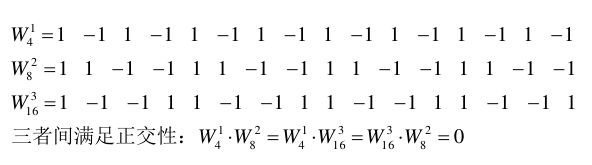
\includegraphics[width=0.7\linewidth]{figures/OVSP}
	\caption{}
	\label{fig:ovsp}
\end{figure}
\subsubsection{地址码}
\begin{itemize}
	\item 区分用户:gold和m
	\item 区分基站:gold
	\item 区分信道:walsh和ovsf
\end{itemize}
\subsection{直接扩频}
扩频:将原始信号于扩频码相乘。\textbf{信号功率下降到原来的1/N}
\begin{figure}[H]
	\centering
	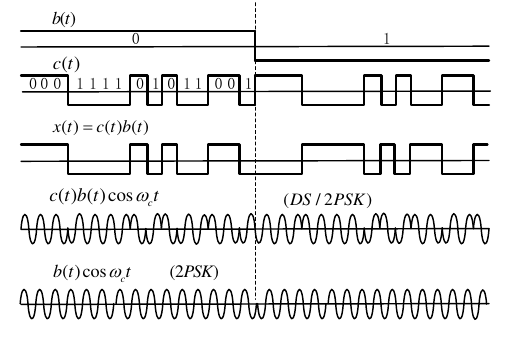
\includegraphics[width=0.7\linewidth]{figures/zhijiekuopin.png}
	\caption{直接扩频}
\end{figure}
\begin{figure}[H]
	\centering
	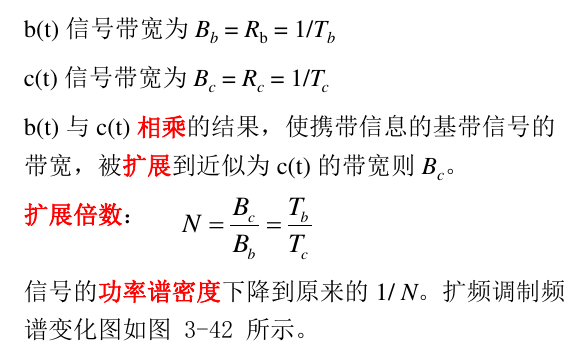
\includegraphics[width=0.7\linewidth]{figures/zhijiekuopin2.png}
	\caption{text}
\end{figure}
解扩:乘以相对应的PN码,还原。
\begin{figure}[H]
	\centering
	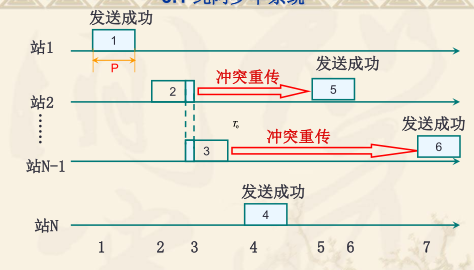
\includegraphics[width=0.9\linewidth]{figures/screenshot002}
	\caption{}
	\label{fig:screenshot002}
\end{figure}
解调方式两种:
\begin{enumerate}
	\item 将Combined信号分别乘上各扩频信号即可得到各路信号。(分离)。适用\textbf{已同步}。
	\item 将扩频信号i分别乘上各扩频信号,得到自相关性强的即为原信号,抖动信号则不是原始信号,适用\textbf{非同步}。
\end{enumerate}
\subsubsection{直接扩频的抗干扰能力}
扩频信号的重要特点:\textbf{抗窄带干扰能力强}
设i(t )为一窄带干扰信号,其频率接近信号的载波频率。
解扩后最终扩频系统的输出干扰功率是输入干扰功率的
1/N ,即扩频系统的处理增益为$ Gp = P_i/P_o = T_b /T_c = N $

\begin{figure}[htbp]
	\centering
	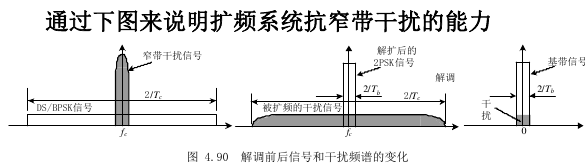
\includegraphics[width=0.9\linewidth]{figures/kangzaidainengli.png}
	\caption{}
	\label{fig:}
\end{figure}
扩频信号对窄带干扰的抑制作用在于接收机
对信号的解扩的同时,对干扰信号的扩频,这降
低了干扰信号的功率谱密度。\\

\section{RAKE接收机}
 利用扩频码的良好自相关特性可以很好地
抑制多径传输带来的干扰 ,当\textbf{多径时延大于扩频码的码片}(时间分集)
的时候 。这些信号 都携带 相同 的
信息 , 利用这些能量 , 则可以
变害为利 , 改善接收信号的质量 
\subsubsection{抗多径干扰}
\begin{itemize}
	\item 利用PN尖锐的自相关特性,很高的码片速率。
	\item  有效抑制与 PN 序列不同步的多径信号分量的干扰
\end{itemize}
\subsubsection{接收方式比较}
\begin{figure}[htbp]
	\centering
	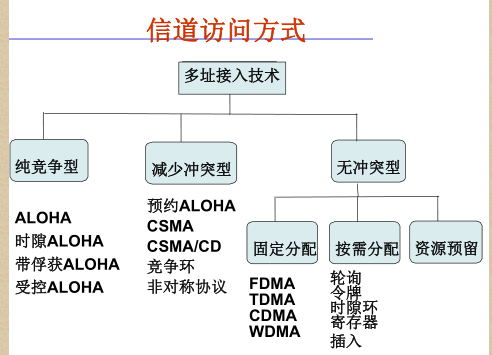
\includegraphics[width=0.7\linewidth]{figures/screenshot001}
	\caption{}
	\label{fig:screenshot001}
\end{figure}
\subsubsection{RAKE接收实现方式}
利用扩频信号设计将各条信号进行\textbf{分离(码片速率小于多径时延差)}。再利用RAKE接收将分离的各条路径信号\textbf{相位校准、幅度加权},将矢量和变为代数和。\\
RAKE接收的本质:时间分集(多径产生时延差)、多径分集、频率分集(扩频带宽远大于相关带宽)。
\section{跳频扩频通信系统}
本质是频率分集。依靠“躲避”来提升抗干扰能力。抗多径、抗同频道干扰、抗衰落。

%	\chapter{通信网结构}
\section{图论基础}
\subsection{一笔画问题}
\textbf{奇点:}与该条边连接的个数有奇数个\\
\textbf{偶点:}与该条边连接的个数有偶数个\\
一笔画定理:
\begin{itemize}
	\item 中间点一定是偶数点
	\item 最多有两个奇点
	\item 若由偶点组成的连通图,一定可以一笔画,以任意点为起点一以这个点为终点
	\item 只有两个奇点的连通图,一定可以一笔画完;画时以一个奇点为起点,另一个奇点为终点。
\end{itemize}
\subsection{图的基础知识}
\subsubsubsection{基础概念}
\begin{itemize}
	\item 相邻点: vi与vj 互为相邻点( vi 和vj 是一条边的两个端点)
	\item 相邻边:两条边与同一端点相关联,则这两条边为相邻边
	\item 度数(或次数):与同一端点相关联的边的个数
	\item 两个端点重合为一点的边成为自环。
	\item 并行边,与同一队端点关联的两条边或两条以上的边
	\item 简单图与复杂图,没有自环和并行边的图称为简单图,否则称为复杂图
	\item 空图:没有点
	\item 孤立点:有点但无边
	\item 平面图和非平面图:非平面图画在平面上时,至少有两条边要相交。平面图则不想交	
\end{itemize}
\subsubsubsection{图的运算}
\begin{itemize}
	\item 并图
	\begin{figure}[H]
		\centering
		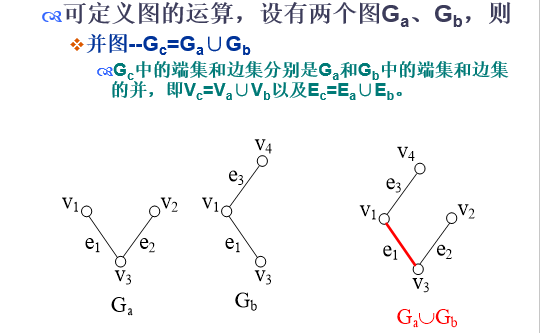
\includegraphics[width=0.5\linewidth]{figures/screenshot039}
		\caption{}
		\label{fig:screenshot039}
	\end{figure}
	\item 交图 
	\begin{figure}[H]
		\centering
		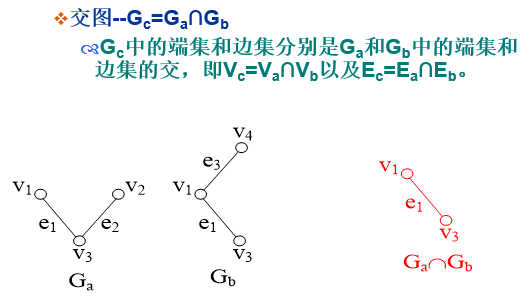
\includegraphics[width=0.5\linewidth]{figures/screenshot040}
		\caption{}
		\label{fig:screenshot040}
	\end{figure}
	\item 差图
	 \begin{figure}[H]
		\centering
		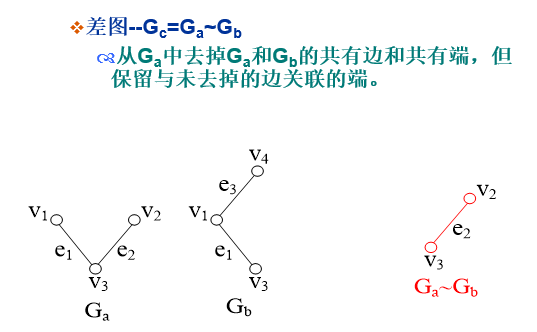
\includegraphics[width=0.7\linewidth]{figures/screenshot041}
		\caption{}
		\label{fig:screenshot041}
	\end{figure}
	一般来说:$ G_a ~ G_b = G_a - G_a\cap G_b $ ,所以该运算要分方向
	\item 环合图
	\begin{figure}[H]
		\centering
		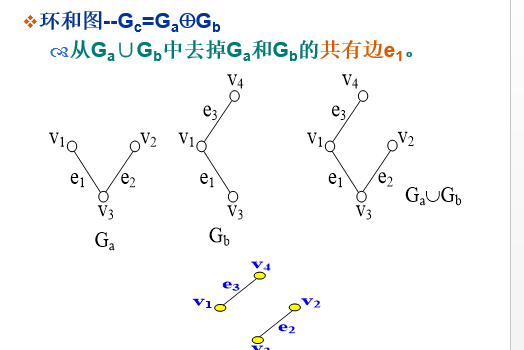
\includegraphics[width=0.7\linewidth]{figures/screenshot042}
		\caption{}
		\label{fig:screenshot042}
	\end{figure}
\end{itemize}
\subsubsection{图的联结性}
\begin{description}
	\item[1.端的度数] 与端相关的变数为该端的度数,自环度数+2.在有向图中\textbf{$ d^+(v_i) $表示离开}$ v_i $的边数,\textbf{$ d^-(v_i) $表示进入},$ v_i $的度数。
\end{description}
\textbf{图的度数性质:}
对于有n个端,m条边的无向图
\begin{equation}\label{key}
\sum_{i=1}^{n}d(v_i) = 2m
\end{equation}
若G为有向图
\begin{equation}\label{key}
\sum_{i=1}^{n}d^+(v_i) = \sum_{i=1}^{n}d^-(v_i) = m
\end{equation}
任意图中,\textbf{度为奇数数的端的数目必为偶数}。
\subsubsection{链、径和还}
\begin{description}
	\item[边序列] 有限条边的一种串序排列称为边序列,要求相邻两边有公共端。(边可重复)
	\item [链] 没有重复边的链
	\item [环] 起点和终点为同一端的链
	\item[径] 无重复边、无重复端的边序列
\end{description}
\subsubsection{连接图}
\textbf{联结图的一般定义}:图内任何2个端之间至少有一条径,这图就称为联结图(或称连通图)。否则就是非联结图(或非连通图)\\
非连接图总可以分为几个部分,所谓部分是指原图的一个子图,该子图\textbf{是一个最大连接图}
\begin{figure}[H]
	\centering
	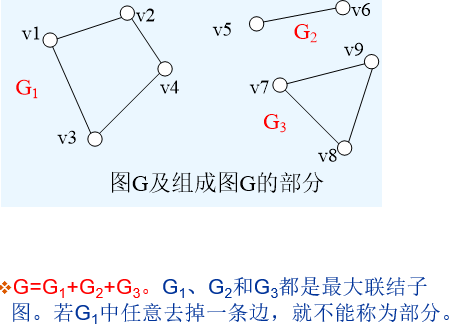
\includegraphics[width=0.7\linewidth]{screenshot003}
	\caption{}
	\label{fig:screenshot003}
\end{figure}
\subsubsection{几种特殊的连接图}
\begin{enumerate}
	\item \textbf{全连接图}:任意两端都有边的无向图成为全连接图各端的度数均为d(vi)=n-1,。其边m和端n的关系
	\begin{figure}[H]
		\centering
		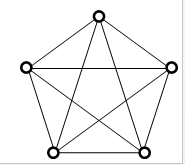
\includegraphics[width=0.3\linewidth]{figures/screenshot046}
		\caption{}
		\label{fig:screenshot046}
	\end{figure}
	
	\begin{equation}\label{key}
	m = C_n^2 = \frac{n(n-1)}{2}
	\end{equation}
	\item \textbf{两部图}:端点集合可分为2个部分,所有边的2个邻端分别在这2个集合中。特别,\textbf{完全两部图}Km,n的端点集合有2个部分,分别有m和n个端点;从2个端集合中各任取一个端,它们之间都有一条边,共有mn条边。
	\begin{figure}[H]
		\centering
		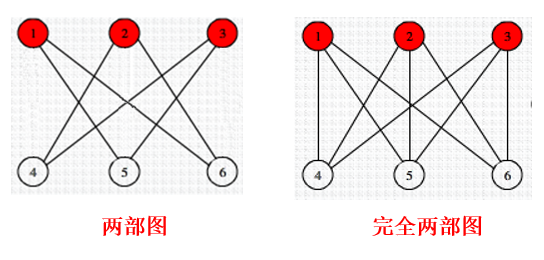
\includegraphics[width=0.7\linewidth]{figures/screenshot047}
		\caption{}
		\label{fig:screenshot047}
	\end{figure}
	
	\item 正则图:所有段的度数都相等.正则图的联结性最均匀;无重边和自环的全联结图是正则图。
	\begin{figure}[H]
		\centering
		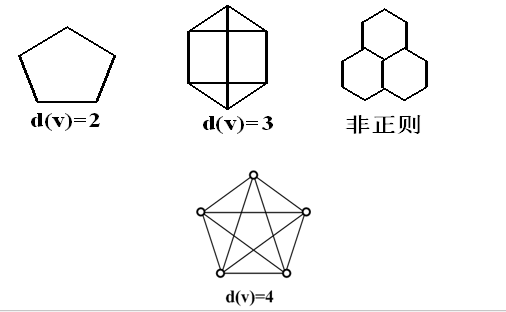
\includegraphics[width=0.7\linewidth]{figures/screenshot048}
		\caption{}
		\label{fig:screenshot048}
	\end{figure}
	
	\item 欧拉图:端度数均为偶数(不一定为连接图)。\\
连接欧拉图<=>存在一个含全边的环	
\begin{figure}[H]
	\centering
	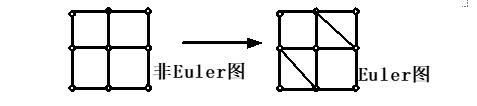
\includegraphics[width=0.7\linewidth]{figures/screenshot049}
	\caption{}
	\label{fig:screenshot049}
\end{figure}
	\begin{figure}[H]
		\centering
		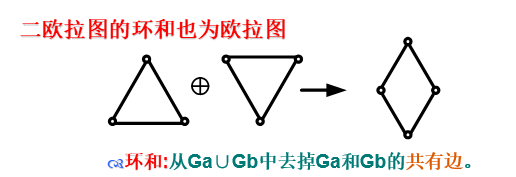
\includegraphics[width=0.7\linewidth]{figures/screenshot050}
		\caption{}
		\label{fig:screenshot050}
	\end{figure}
	
	\item M图:如果图中只有2个度数为奇数的端,则此图称为M图。\\
	M图可以是联结图,也可以是非联结图,但此时各部分除一个是M图外,其他都是欧拉图。
	\begin{figure}[H]
		\centering
		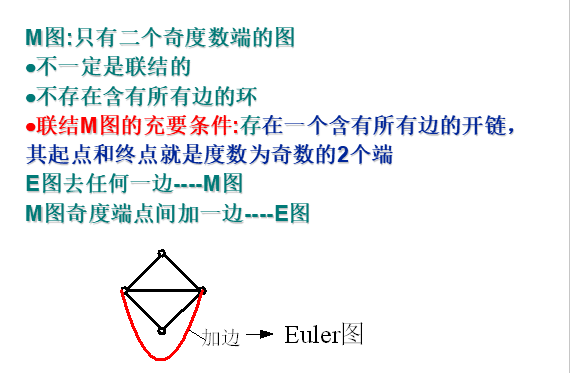
\includegraphics[width=0.7\linewidth]{figures/screenshot051}
		\caption{}
		\label{fig:screenshot051}
	\end{figure}
	
	\item 汉密尔顿(Hamilton)图:当图中至少存在一个含有所有端的环,这个图称为汉密尔顿图(也称哈密顿图),上述的环称为汉密尔顿环。
	\begin{figure}[H]
		\centering
		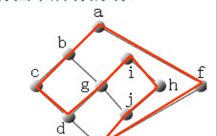
\includegraphics[width=0.7\linewidth]{figures/screenshot052}
		\caption{}
		\label{fig:screenshot052}
	\end{figure}
	
\end{enumerate}

\section{树}
定义:任何二端间有径且只有一条径的图
\subsection{基本性质}
\begin{enumerate}
	\item 树是无环的连接图
	\item 树是最小连通图。去掉任意一边就变成非连接图
	\item 若树有m条边及n个端,则有\textbf{m=n-1}
	\item 除单点树外,树\textbf{至少有2个端的度数为1}
\end{enumerate}
\subsection{树的一些概念}
\begin{figure}[H]
	\centering
	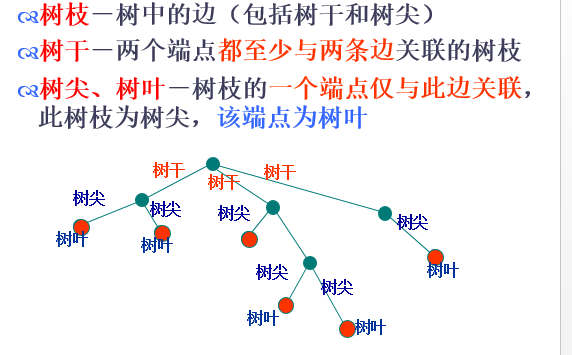
\includegraphics[width=0.7\linewidth]{figures/screenshot053}
	\caption{}
	\label{fig:screenshot053}
\end{figure}

\subsection{主树}
生成树:包含所有端点,\textbf{一定为连通图},可能不止一个
\subsection{树枝与连枝}
对于图的某一棵主树而言,主树上的边称为树枝,非树枝的边称为连枝。
主树就是树枝集;
连枝的边集称为连枝集或称为树补。
\subsection{图G的阶及其空度
}
\subsubsection{阶}
联结图G的主树T的树枝数称为图G的阶。
若图G有n个端,则它的阶$ \rho $为
$ \rho $(G)=$ \rho$=| T|=mT=n-1
\subsubsection{空度}
联结图G的连枝集的连枝数称为图G的空度,记为$ \mu $。
当G有m条边时,有\textbf{$  \mu(G)=|G-T|=m-n+ $1} 且 $ \rho+\mu=m $
\begin{itemize}
	\item $ \mu $越大,连枝数越多,图G的联结性越好。
	\item $ \mu = 0 $表示最低联结性,即G是最小连接图。
\end{itemize}
\subsubsection{主林与林补}
对一个非联结图G,它可分成k个部分,也就是k个最大联结图。每个部分至少有一棵主树。这可找到k棵主树,所形成的集称为主林。余下的边所形成的集称为林补。
此时,G的阶可定义为主林的边数,G的空度为林补的边数。
\begin{equation}\label{key}
\rho(G)=(n1-1)+(n2-1)+….+(nk-1)=n-k 
\end{equation}
\begin{equation}\label{key}
\mu(G)=m-n+k \\
\end{equation}

\section{割和环}
\subsection{割}
割是指图的某些子集,\textbf{去掉这些子集就使图的部分数增}加。若图是联结的,去掉这种子集就成为非联结图。\\
根据这种子集的元素不同,可分为割端集和割边集。
\subsubsection{割端与割端集}
\subsubsubsection{割端}
\textbf{割端:}令v是G的一个端,在去掉v和与之关联的边后,若使G的部分数增加,则称v是G的割端。
\subsubsubsection{割端集}
\textbf{割端集}:去掉几个端后,部分数增加,则这些端的集称为割端集。\\
\textbf{最小割端集中的端数},称为图的联结度,表示要破坏图的联结性的难度;联结度愈大,联结性愈不易被破坏。
\subsubsection{割边集和割集}
\textbf{割边集}:令S是联结图G的边子集,如果在G中去掉S能使G成为非联结图,则称S是G的割边集\\
\textbf{割集,最小割边集}:\textbf{若S的任何真子集都不是割边集},称S是割集。
实际上\textbf{,割集是最小割边集}。\\
\textbf{最小割集的边数称为图的结合度,表示图的联结程度。}
\begin{figure}[H]
	\centering
	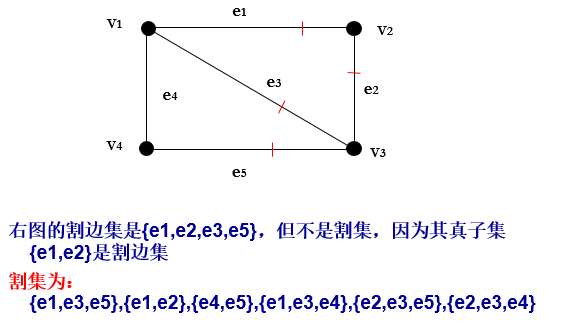
\includegraphics[width=0.7\linewidth]{figures/screenshot054}
	\caption{}
	\label{fig:screenshot054}
\end{figure}

\subsection{联结度、结合度、连通度}
\begin{itemize}
	\item 联结度:最小割端集的端数称为图的联结度。
	\item 结合度:最小割集的边数称为图的结合度。
	\item 连通度:联结度和结合度统称为连通度。
\end{itemize}
\textbf{联结度是点连通度;
结合度是边连通度}
对于通信网来说,连通度越高,可靠性越好
\subsection{基本割集}
设T是联结图G的一棵主树,取一条树枝与\textbf{某些连枝}一定能构成一个割集,这种割集称为基本割集。\\
\textbf{基本割集只含一条树枝}\\
若G有n个端,则主树有n-1条树枝,所以有$ n-1 $个基本割集\\
基本割集有$ n-1 $,由基本割集及其\textbf{环和}共形成$ 2^(n-1)-1 $(二项式求和),然后排除重复的地方。                                \begin{figure}[H]
	\centering
	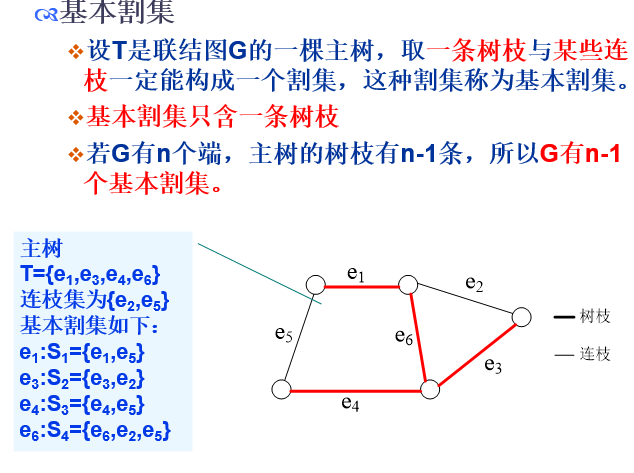
\includegraphics[width=0.7\linewidth]{figures/screenshot045}
	
	\caption{}
	\label{fig:screenshot045}
\end{figure}
\begin{figure}[H]
	\centering
	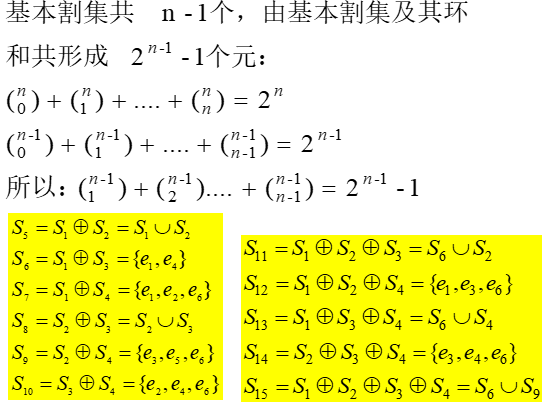
\includegraphics[width=0.7\linewidth]{figures/screenshot056}
	\caption{}
	\label{fig:screenshot056}
\end{figure}
\begin{enumerate}
	\item $ C_4^1 $
		\item $ C_4^2 $
			\item $ C_4^3 $
				\item $ C_4^4 $
\end{enumerate}
\textbf{再去掉所有基本割集的并或者重复的。}
 \subsection{基本环和所有环的方法}                              
取一条连枝可与某些树枝构成\textbf{闭径或环}。这种仅包含有一条连枝的环称为联结图的\textbf{基本环}。显然,基本环的数目等于连枝数\textbf{m-n+1}。
基本环的环和可组成$ 2^{m-n+1}-1 $个元,每个元或为环,或为环的并。
\begin{figure}[H]
	\centering
	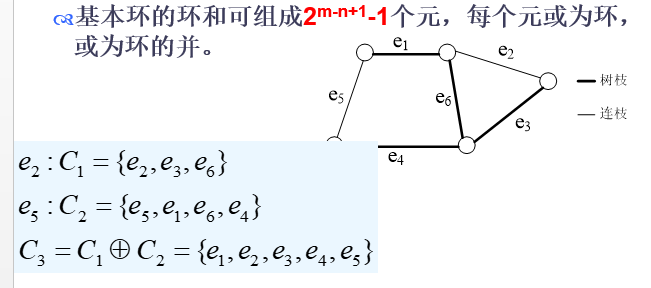
\includegraphics[width=0.7\linewidth]{figures/screenshot044}
	\caption{}
	\label{fig:screenshot044}
\end{figure}

\section{平面性和对偶性}
平面图,任意两条边无交点(除端点)。
\subsection{平面型}
\begin{itemize}
	\item 设一个联结的平面图有m条边,n个端,把平面分成S个区域(包括开区域),它们之间有$ S=m-n+2 $。
	\item 对于无重边、无自环的联结图,具有平面性的必要条件是$ m\le 3n-6 $(即平面图必定有$ m\le 3n-6 $ ,但$ m\le 3n-6 $ 不一定是平面图)。
\end{itemize}
\subsection{对偶性}
设有两个边集E相同的图G1和G2,若G2中每个无重复端的环(闭径)都对应G1中的一个割集,反之亦然,则G1和G2互为对偶图或具有对偶性。
\begin{itemize}
	\item \textbf{平面图的对偶图总是存在的,而非平面图是没有对偶图的}。
	\item 倘若一个图G的对偶图就是自己,则称G为自对偶图。
	
\end{itemize}
\begin{figure}[H]
	\centering
	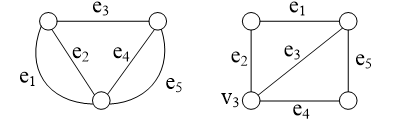
\includegraphics[width=0.7\linewidth]{figures/screenshot057}
	\caption{}
	\label{fig:screenshot057}
\end{figure}
\begin{figure}[H]
	\centering
	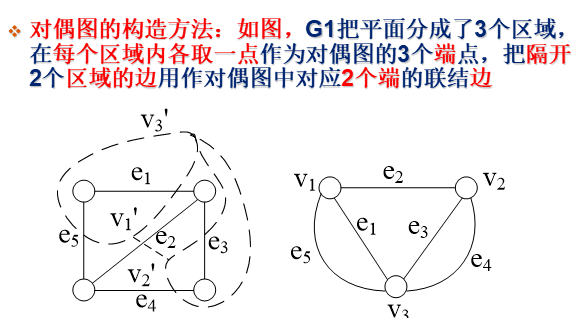
\includegraphics[width=0.7\linewidth]{figures/screenshot058}
	\caption{}
	\label{fig:screenshot058}
\end{figure}
\section{图阵}
\subsection{关联阵}
\subsubsection{全关联阵}
\begin{figure}[H]
	\centering
	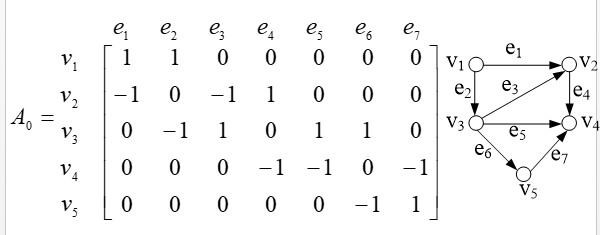
\includegraphics[width=0.7\linewidth]{figures/screenshot060}
	\caption{}
	\label{fig:screenshot060}
\end{figure}
\begin{figure}[H]
	\centering
	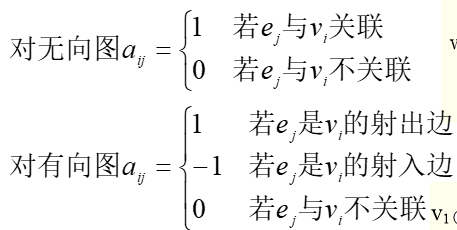
\includegraphics[width=0.7\linewidth]{figures/screenshot061}
	\caption{}
	\label{fig:screenshot061}
\end{figure}
\begin{itemize}
	\item 每行中非零元素的个数等于该端的度数
	\item 每一列元素之和为对无向图为2,对有向图为0
\end{itemize}
\subsubsection{关联阵}
\textbf{去掉全关联阵中的任一行即得关联阵}
\begin{itemize}
	\item 联结图的关联矩阵中,必存在至少一个(n-1) ×(n-1)的方阵是非奇异的,这个方阵所对应的边集就是一棵主树。
	\item 若关联矩阵中有一个(n-1) ×(n-1)的方阵是奇异的,即它的行列式值为零,则这方阵所对应的边集中必存在环。
	\item 当关联矩阵的阶小于n-1时,它所对应的图必为非联结图,因为没有(n-1) ×(n-1)的方阵是非奇异的,也就是不存在主树。
\end{itemize}
\textbf{联结图主树数目S与全关联阵的关系
}\begin{equation}\label{key}
S = |AA^T|
\end{equation}
\begin{figure}[H]
	\centering
	\includegraphics[width=0.7\linewidth]{figures/screenshot062}
	\caption{}
	\label{fig:screenshot062}
\end{figure}
\begin{itemize}
	\item AAT(无重复边)对角线上的元是端的度数(A0中没有删的行所对应的端),其他元非-1即零(若两个端之间没有边,为零,有边为-1)。
	\item 对于无向图,可以在图上任意加箭头,得相应的有向图,这样就可以求得无向图的主树数目.
\end{itemize}
\subsection{割阵}
\begin{figure}[H]
	\centering
	\includegraphics[width=0.7\linewidth]{figures/screenshot064}
	\caption{}
	\label{fig:screenshot064}
\end{figure}
S1,S2,S3,S4为基本割集。\textbf{正负1看树枝所指端,如果边枝和树枝指向相同则为正,反之为负}
\begin{figure}[H]
	\centering
	\includegraphics[width=0.7\linewidth]{figures/screenshot065}
	\caption{}
	\label{fig:screenshot065}
\end{figure}
\begin{figure}[H]
	\centering
	\includegraphics[width=0.7\linewidth]{figures/screenshot066}
	\caption{}
	\label{fig:screenshot066}
\end{figure}
\textbf{联结图的环阵B和割阵Q以下关系,若边的次序是一样的: $ BQ^T $=0
}
\subsection{邻接阵}
\begin{figure}[H]
	\centering
	\includegraphics[width=0.7\linewidth]{figures/screenshot067}
	\caption{}
	\label{fig:screenshot067}
\end{figure}
\section{最短径问题}
\subsection{最短主树}
\subsubsection{无限制条件}
\subsubsubsection{P算法
}
\begin{figure}[H]
	\centering
	\includegraphics[width=0.7\linewidth]{figures/screenshot068}
	\caption{}
	\label{fig:screenshot068}
\end{figure}
\subsubsubsection{K算法}
\begin{figure}[H]
	\centering
	\includegraphics[width=0.7\linewidth]{figures/screenshot069}
	\caption{}
	\label{fig:screenshot069}
\end{figure}
\subsubsubsection{破圈法}
\begin{figure}[H]
	\centering
	\includegraphics[width=0.7\linewidth]{figures/screenshot070}
	\caption{}
	\label{fig:screenshot070}
\end{figure}
\subsubsection{有限制条件下最短树的求取
}
\subsubsubsection{穷举法(可用置换法)
}

\subsubsubsection{E-W算法}
\subsection{端间的最短径}
\subsubsection{D算法}
\begin{figure}[H]
	\centering
	\includegraphics[width=0.7\linewidth]{figures/screenshot071}
	\caption{}
	\label{fig:screenshot071}
\end{figure}
\subsubsection{F算法}
十字交叉法,加上一个中转矩阵(每次更新时,更新中转矩阵即可)
\subsection{次短径和可用径
}
\begin{figure}[H]
	\centering
	\includegraphics[width=0.7\linewidth]{figures/screenshot072}
	\caption{}
	\label{fig:screenshot072}
\end{figure}
\subsubsection{找与最短径边分离的次短径}
当用F算法或D算法得到最短径后\textbf{,从原图中去掉此径的所有边(保留这边的两个端}),然后在剩下的图中\textbf{用D算法求vs和vt间的最短径}。这就是所要求的次短径。这方法还可继续下去。
\subsubsection{找与最短径端分离的最短径。
}
在这种情况下,求得最短径后\textbf{,应把径中的所有中间端去掉(同时也去掉与之关联的边)},在余下的图中求vs和vt间最短径,就得到与最短径分离的次短径。这方法也可继续下去。
\subsection{限制条件下的可用径}
\begin{enumerate}
	\item 用F算法求得图的最短径长矩阵W和转接矩阵R
	\item DFS遍历各点,在进行判定。
\end{enumerate}
\begin{figure}[H]
	\centering
	\includegraphics[width=0.7\linewidth]{figures/screenshot073}
	\caption{}
	\label{fig:screenshot073}
\end{figure}
\section{网的中心和中点}
\subsection{网中心}
Steps:
\begin{itemize}
	\item wij有一最大值;称为最长的最短径.\textbf{求每个端点到其它端点的最大长度}
	\item ti的最小值所对应的端vi*称为网的中心.求上述长度的最小值,所对应的点设置为中心。
\end{itemize}
\begin{figure}[H]
	\centering
	\includegraphics[width=0.7\linewidth]{figures/screenshot074}
	\caption{}
	\label{fig:screenshot074}
\end{figure}
\subsection{网中点}
Steps:
\begin{itemize}
	\item 按行求和
	\item 上述的最小值所对应的点
\end{itemize}
\textbf{网的中点可用作全网的交换或控制中心}
\begin{figure}[H]
	\centering
	\includegraphics[width=0.7\linewidth]{figures/screenshot075}
	\caption{}
	\label{fig:screenshot075}
\end{figure}
例题:
\begin{figure}[H]
	\centering
	\includegraphics[width=0.7\linewidth]{figures/screenshot076}
	\caption{}
	\label{fig:screenshot076}
\end{figure}
\section{站址问题}
\subsection{单中点问题
}
设有n个用户点,它们的平面坐标分别为(xi,yi)(i=1,2,…,n)。又设各点的加权系数为wi,代表用户所需的联线数或其它需求的大小。单中点问题就是要找到一个中点的坐标(xq,yq),使代价L最小。
\begin{equation}\label{key}
L = \sum{i}{} w_id_i
\end{equation}
$ d_i $为距离的测度
\begin{enumerate}
	\item 欧式距离,平方和求根
	\item 距离平方,欧式距离的平方。适合电磁场传播
	\item 矩形距离,直角边的距离。适合城市街道铺设
\end{enumerate}
\textbf{欧式距离或者平方下},中心站点的最小距离几何确定法:\\
可以证明,中点的位置,是距离三个点位置最近的中心点,按照初等几何的原理,应该是该点与三个点的连线形成的夹角,均为120度。
\begin{figure}[H]
	\centering
	\includegraphics[width=0.7\linewidth]{figures/screenshot077}
	\caption{}
	\label{fig:screenshot077}
\end{figure}
斯顿树:如容许增加新的端点,包括中心点,存在比以前的最短主树更短的主树。这种主树称为斯顿树。\\
\vspace{1pt}
\textbf{矩形线距离的情况}
理论基础:
\begin{figure}[H]
	\centering
	\includegraphics[width=0.7\linewidth]{figures/screenshot078}
	\caption{}
	\label{fig:screenshot078}
\end{figure}
几种情况:
\begin{figure}[H]
	\centering
	\includegraphics[width=0.7\linewidth]{figures/screenshot079}
	\caption{}
	\label{fig:screenshot079}
\end{figure}
\begin{figure}[H]
	\centering
	\includegraphics[width=0.7\linewidth]{figures/screenshot080}
	\caption{}
	\label{fig:screenshot080}
\end{figure}

\subsection{k中点问题}
一般所谓的k中点问题,是指k为预给值,\textbf{不计各中点的中继线代价,求这些中点的位置,以使总代价最小}。
\begin{equation}\label{key}
L = \sum_{i,j}^{} c_{ij}w_jd_j
\end{equation}
$ c_{ij} $表示i,j是否有连接。
类似\textbf{k-means}算法。先随机确定初始点,之后根据测度进行k聚类,更新中点,判定误差。
\subsection{设站问题}
\begin{figure}[H]
	\centering
	\includegraphics[width=0.7\linewidth]{figures/screenshot081}
	\caption{}
	\label{fig:screenshot081}
\end{figure}
单,双,三中点分别计算。得到一个关于设站成本f的图形。再进一步分析
\begin{figure}[H]
	\centering
	\includegraphics[width=0.7\linewidth]{figures/screenshot082}
	\caption{}
	\label{fig:screenshot082}
\end{figure}









	\chapter{WCDMA 移动通信系统}
\section{WCDMA 系统概述}
三种方案对比,详细见书P186。
\subsection{WCMDA的发展}
GSM->GPRS->EDGE->WCDMA->HSDPA->HSUPA>LET\\
详细演进版本可见P187。
\subsection{WCMDA系统结构}
无线接入 网负责处理所有与无线通信相关的
功能。而 CN 则采用了 GSM/GPRS 的定义,这样可
以实现网络的平滑过渡,核心网负责对话音及
数据业务进行交换和路由查找,以便将业务连
接至外部 网络.
\begin{figure}[H]
	\centering
	\includegraphics[width=0.7\linewidth]{figures/screenshot011}
	\caption{}
	\label{fig:screenshot011}
\end{figure}
\begin{enumerate}
	\item UE,UE 完成人与网络间的交互,通过\textbf{ Uu 接口}与无
	线接入网相连,与网络进行信令和数据交换。包
	括两部分:
	\begin{itemize}
		\item ME,移动设备
		\item USIM,UTMS用户识别模块。
	\end{itemize}
	\item 无线接入网(UTRAN),UTRAN 位于两个开放接口 Uu 和 Iu 之间,完成所有
	与无线有关的功能。
	\begin{itemize}
		\item 无线网络控制器( RNC ),主要完成连接建立和断开、切换、宏分集合并
		和\textbf{无线资源管理控制}等功能。
		\begin{enumerate}
			\item 控制 RNC ( CRNC )。对于某个 Node B 来说,直接
			控制它的 RNC 就是\textbf{控制} RNC ( CRNC )
			\item 服务 RNC(SRNC) 。与 CN 有连接,为 UE 提供资源的
			RNC。(越区切换合并)
			\item 漂移 RNC(DRNC) 。把自己的资源借给 SRNC 为某一
			个 UE 使用的(仅一个Node B资源)
		\end{enumerate}
		\begin{figure}[H]
			\centering
			\includegraphics[width=0.7\linewidth]{figures/screenshot012}
			\caption{}
			\label{fig:screenshot012}
		\end{figure}
		\item Node B,Node B 通过 Iub 接口和基站控制器 RNC 互连。它主
		要由接口电路、基带处理单元、射频前端和控制单元
		部分组成。\textbf{ Node B=BBU(基带处理)+RRU(射频前端+ 天馈系统},\textbf{基带处理是核心功能},Node B 还负责完成更软切换、定位测量和执行无
		线资源分配与管理控制指令的功能
	\end{itemize}
	\item  CN 核心网络。
	\begin{itemize}
		\item CS域:MSC/VLR,GMSC
		\item PS域:SGSN,GGSN,CG。
		\item HLR.
	\end{itemize}
	\item 接口
	\begin{enumerate}
		\item Cu,USIM和ME之间
		\item Uu,UE和UTRAN,是UMTS中最重要的开放接口之一。
		\item Iu,UTRAN和CN。
		\item Iur,RNC之间
		\item Iub,Node B之间。
	\end{enumerate}
\end{enumerate}
\subsection{CDMA的优点}
\begin{enumerate}
	\item 抗干扰能力强,特别是抗窄带干扰;
	\item 可检测性低,不容易被侦破
	\item 具有多址能力,易于实现码分多址技术
	\item 可抗多径干扰
	\item 可抗频率选择性衰落
	\item 频谱利用率高,容量大
\end{enumerate}
\subsection{UTRAN 接口协议}
\subsubsection{结构图}
\begin{figure}[H]
	\centering
	\includegraphics[width=0.7\linewidth]{figures/screenshot014}
	\caption{}
	\label{fig:screenshot014}
\end{figure}
特点:
\begin{enumerate}
	\item 所有接口具有开放性
	\item 将无线网络层与传输层分离
	\item 控制面和用户面分离
\end{enumerate}
Iu,Iub,Iur使用\textbf{ATM}承载。
\subsubsection{协议栈}
\textbf{UTRAN 控制面协议栈}是指协议和设备的对应关系
。 \textbf{UE 里面实现的协议是最完备}的,所有的 Node B 只实
现第一层,从 Uu 口的角度来讲,\textbf{ RNC 实现第二层(}从
MAC 到 RRC ),\textbf{ CN 只实现 RRC 之上的}
\begin{figure}
	\centering
	\includegraphics[width=0.7\linewidth]{figures/screenshot015}
	\caption{}
	\label{fig:screenshot015}
\end{figure}
UTRAN 用户面协议栈用户面有 CS 和 PS 域,从 UE的角度讲,没有RRC。
\begin{figure}
	\centering
	\includegraphics[width=0.7\linewidth]{figures/screenshot016}
	\caption{}
	\label{fig:screenshot016}
\end{figure}
\section{WCDMA系统的关键技术}
\subsection{基本技术}
WCDMA 系统发射机和接收机的信号处理流程
\begin{enumerate}
	\item 信源编码 。自适应多 速率 AMR
	技术( 带8 8 种信源 速率) .
	\item 信道编码 、交织,抵抗无线传播环境中的各种衰落。主要采用 卷积码、 Turbo 码和交
	织等信道编码技术
	\item 扩 频、加扰,这两步是 WCDMA 系统所特有的,采用高速的OVSF提高数
	字符号的速率,增加信号带宽
	\item 调制,
\end{enumerate}
\subsection{RAKE接收}
\begin{itemize}
	\item 多径分离
	\item 多径合并准则
	\item  RAKE接收的本质。
\end{itemize}
\subsection{功率 控制技术}
从通信链路的角度,功率控制可 分为
\begin{itemize}
	\item 前向功率控制,基站到移动台
	\item 反向功率控制,移动台到基站
\end{itemize}
从 功率控制方法的角度,功率控制可 分为
\begin{itemize}
	\item 开环功率控制
	\item 闭环功率控制
\end{itemize}
快速 、准确的\textbf{功率 控制技术}是 保证 WCDMA 系统性
能的\textbf{核心 }技术。
\subsubsection{反向开环功率控制}
根据接收到的钱箱链路信号的功率大小来调整自己的发射功率。开环功率控制由于补偿信道中的\textbf{平均路径损耗及慢衰落},有一个很大的\textbf{动态范围}。\\
开环功率控制只能起到粗略控制
的作用 。
\subsubsection{反向闭环 功率控制}
建立于开环功率控制之上,最开环功率控制进行校正。根据反向链路上移动台的信号强弱,产生功率控制指令,通过前向链路将功率指令发送给移动台,移动台根据该指令,在开环功率控制所选择发射功率的基础上,快速校正自己功率。克服\textbf{快衰落}。
\begin{itemize}
	\item 内环功率控制,基站测量移动台的移动台信号,与某个门限比较,进行发送相应的功率控制指令。
	\item 外环功率控制,对内环门限进行调整。
\end{itemize}
\subsection{软切换}











\end{document}